\chapter{Additional Figures}
\label{ap:addFig}
Here we show additional figures.
Some of the figures are repetive and left out in the main chapters, other may provide some details, which are not needed to understand the results but may be intersting and provide a more visual understanding for the coursies reader.
\clearpage
\section{Ozone}
\subsection{Ozone Prior}
\begin{figure}[ht!]
	\centering
	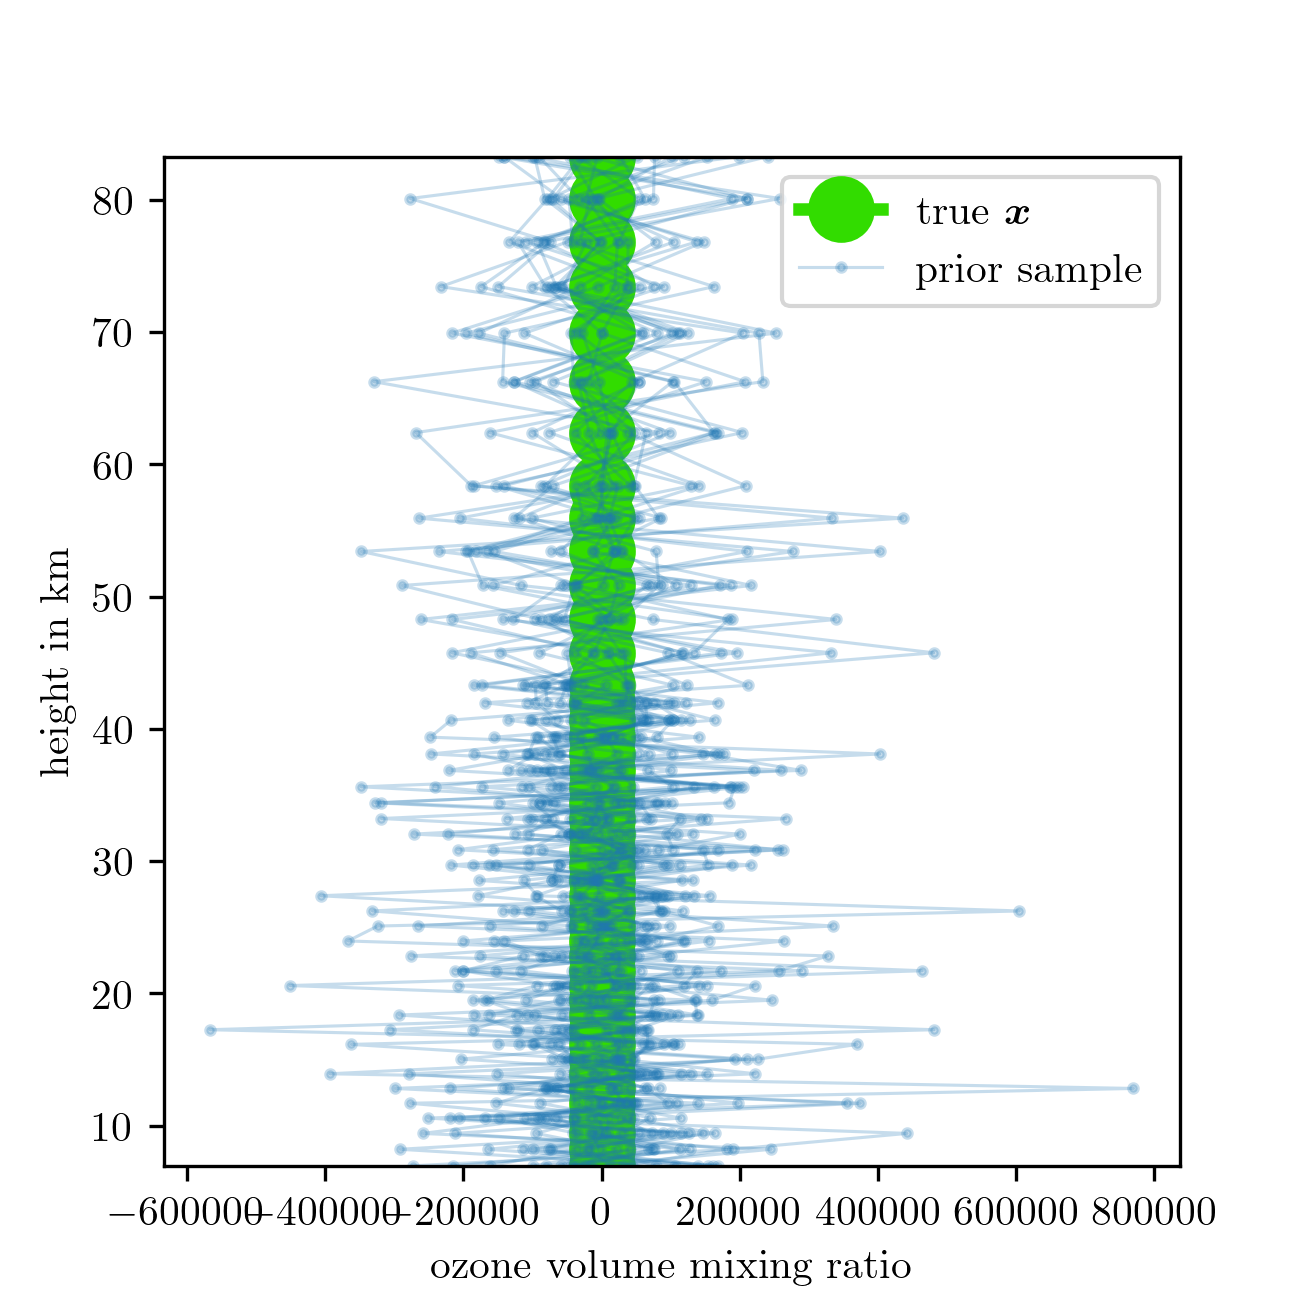
\includegraphics{OzonePrior.png}
	\caption[Samples from ozone prior distribution.]{We draw samples from ozone prior distribution $\bm{x} \sim \mathcal{N}(0,\delta \bm{L})$ after generating a sample from the hyper-prior distribution $\delta \sim \mathcal{T}(1,10^{-10})$. Note that since the variance of prior samples is very large compared to the ozone volume mixing ratios, the ozone profile appears to be constant, which is not the case, see e.g. Fig. \ref{fig:O3Samp}.}
	\label{fig:O3Prior}
\end{figure}
\clearpage
\subsection{Integrated Autocorrelation Plots} 
\begin{figure}[ht!]
	\centering
	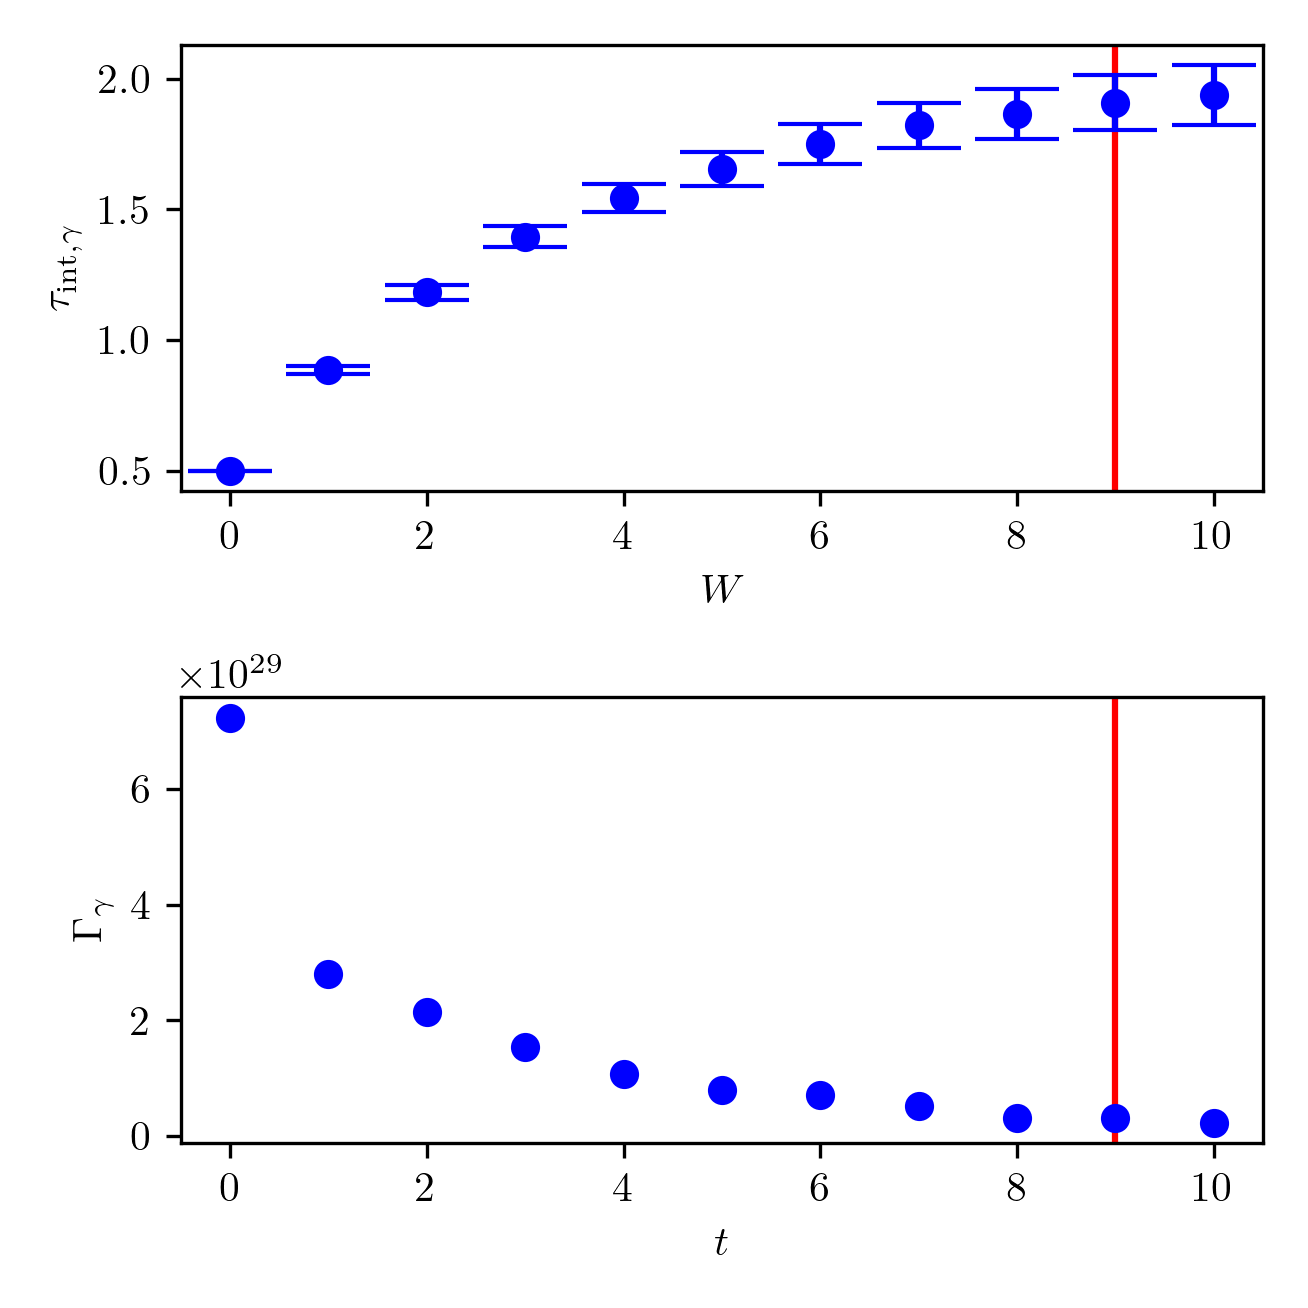
\includegraphics{UwerrTauIntFirstO3gam.png}
	\caption[IACT and autocorrelation of samples $\gamma \sim \pi( \cdot | \bm{y})$, for linear model.]{Provided by \cite{drikHesse}, the IACT $\tau_{\text{int},\gamma}$ at summation windows W as well as the estimated autocorrelation function $\Gamma_{\gamma}$ at lag $t$ of the samples $\gamma \sim \pi(\cdot| \bm{y})$ based on the linear forward model.}
	\label{fig:IATCGamLin}
\end{figure}
\begin{figure}[ht!]
	\centering
	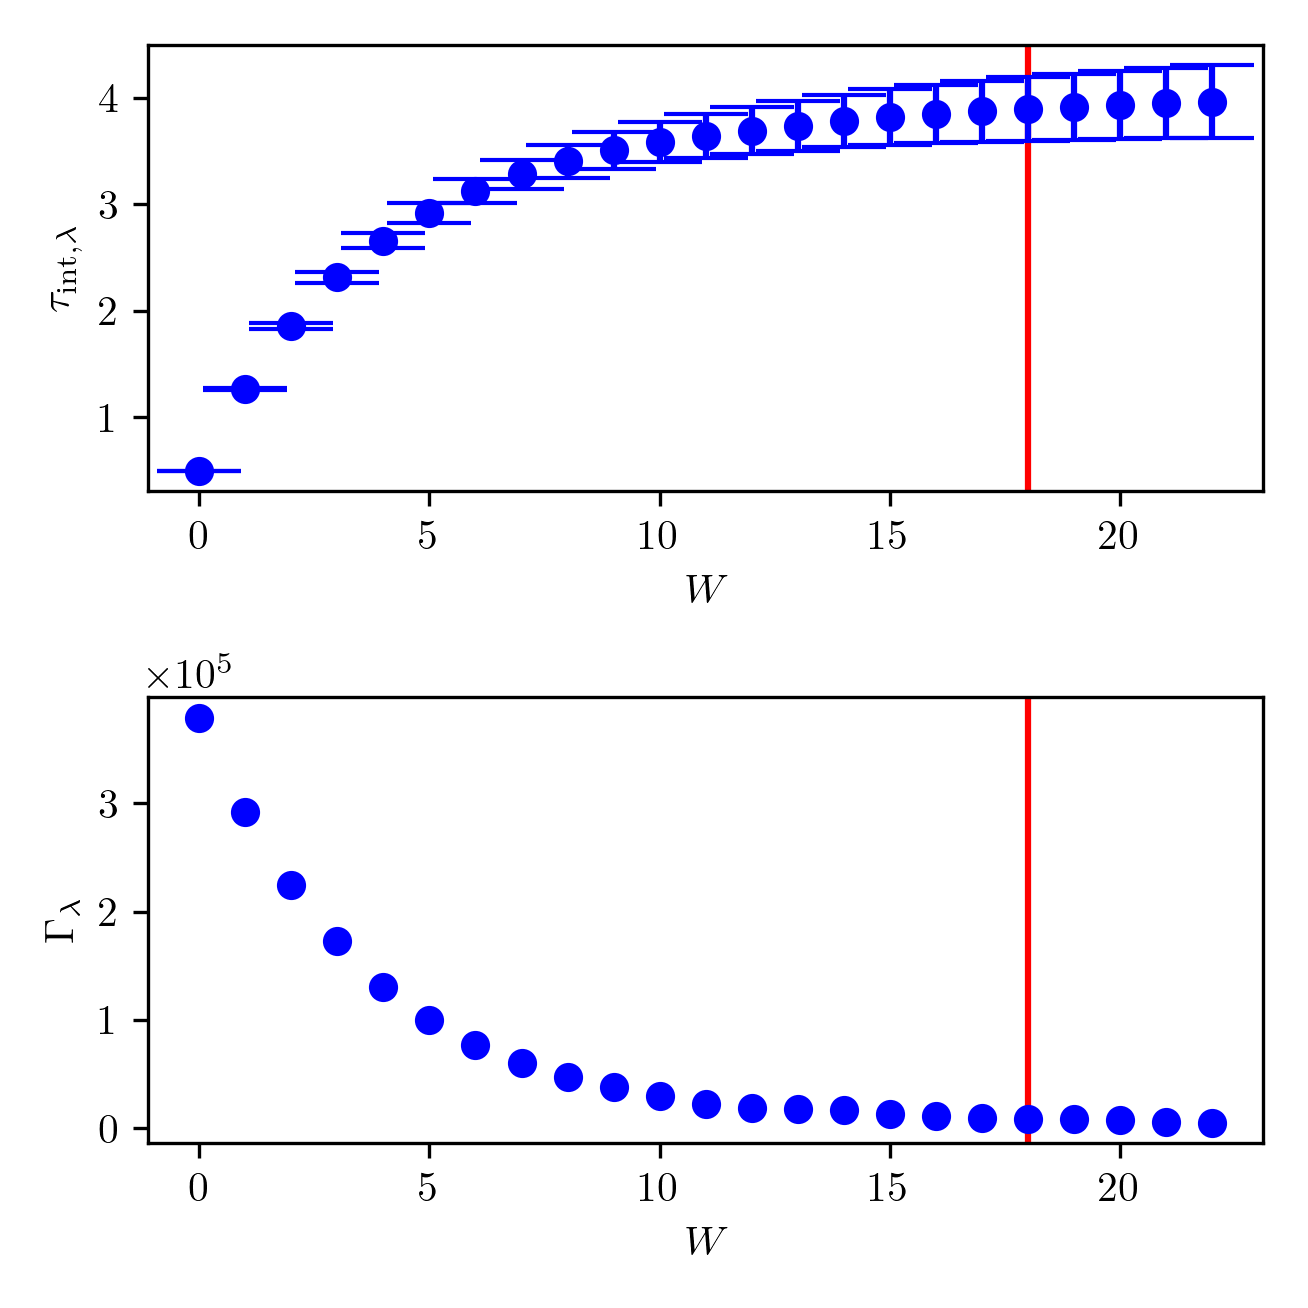
\includegraphics{UwerrTauIntSecO3lam.png}
	\caption[IACT and autocorrelation of samples $\lambda \sim \pi( \cdot | \bm{y})$, for approximated model.]{Provided by \cite{drikHesse}, the IACT $\tau_{\text{int},\lambda}$ at summation windows W as well as the estimated autocorrelation function $\Gamma_{\lambda}$ at lag $t$ of the samples $\lambda \sim \pi( \cdot | \bm{y})$ based on the approximated forward model.}
	\label{fig:IATCSecO3lam}
\end{figure}
\begin{figure}[ht!]
	\centering
	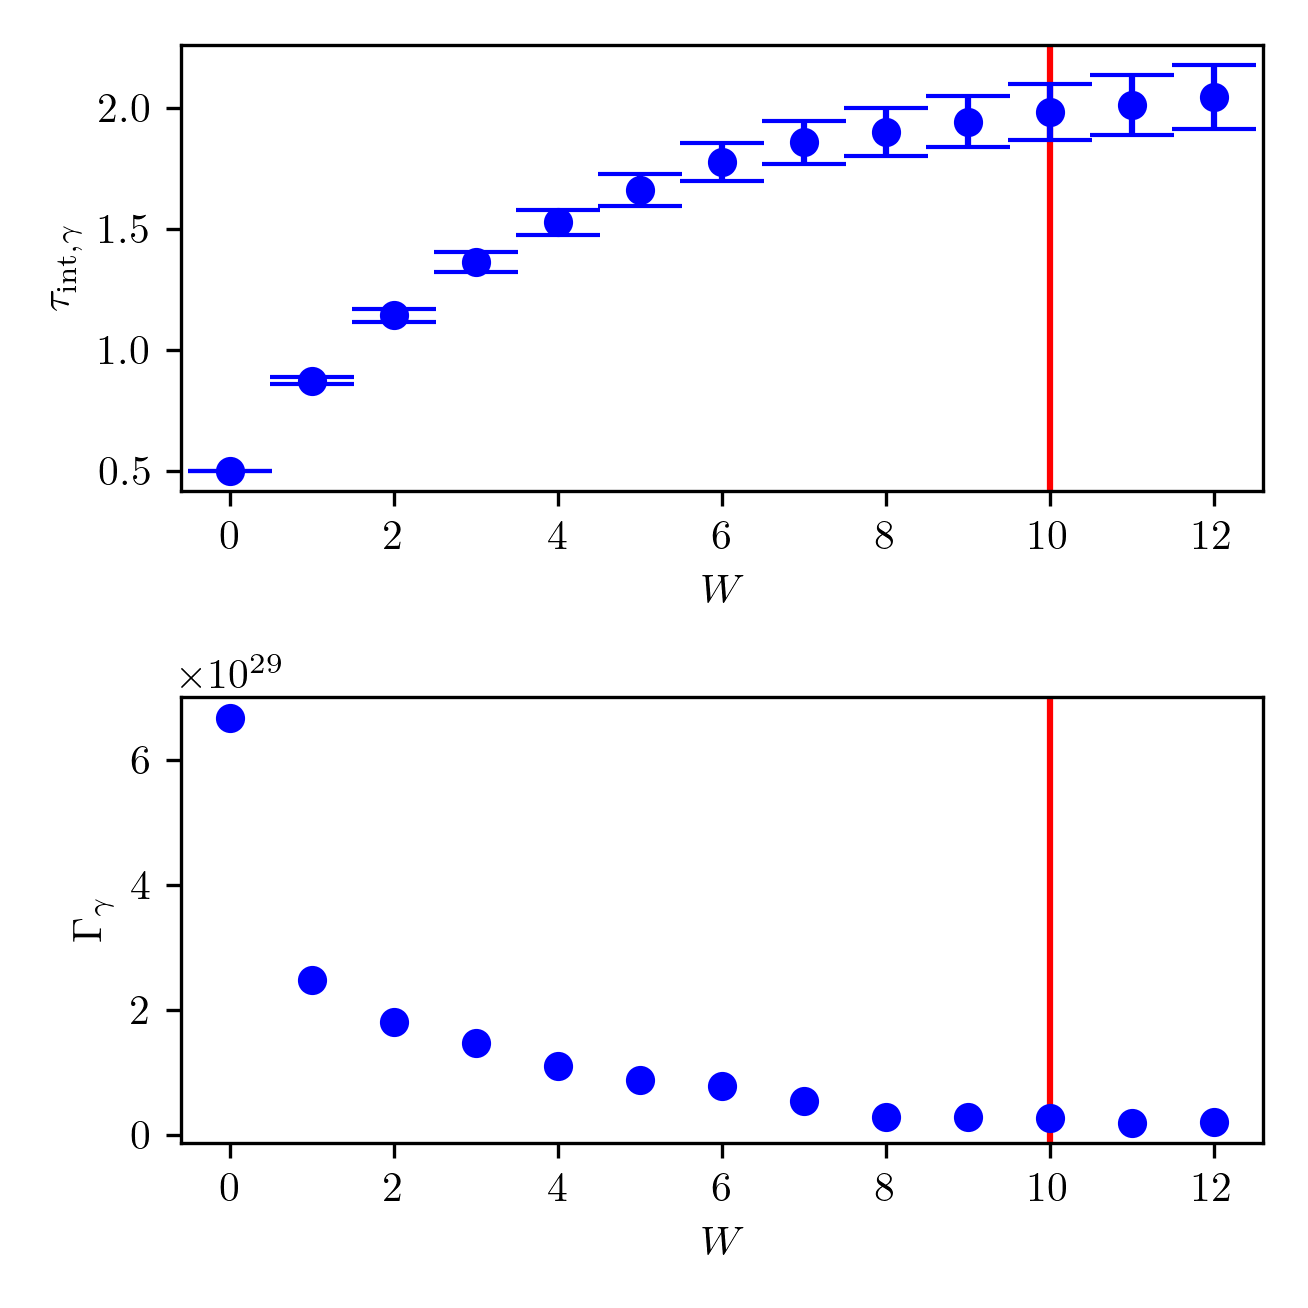
\includegraphics{UwerrTauIntSecO3gam.png}
	\caption[IACT and autocorrelation of samples $\gamma \sim \pi( \cdot| \bm{y})$, for approximated model.]{Provided by \cite{drikHesse}, the IACT $\tau_{\text{int},\gamma}$ at summation windows W as well as the estimated autocorrelation function $\Gamma_{\gamma}$ at lag $t$ of the samples $\gamma \sim \pi( \cdot | \bm{y})$ based on the approximated forward model.}
	\label{fig:IATCSecO3gam}
\end{figure}
\clearpage
\subsection{Eigenvectors of conditional precision matrix}
 \begin{figure}[ht!]
 	\centering
 	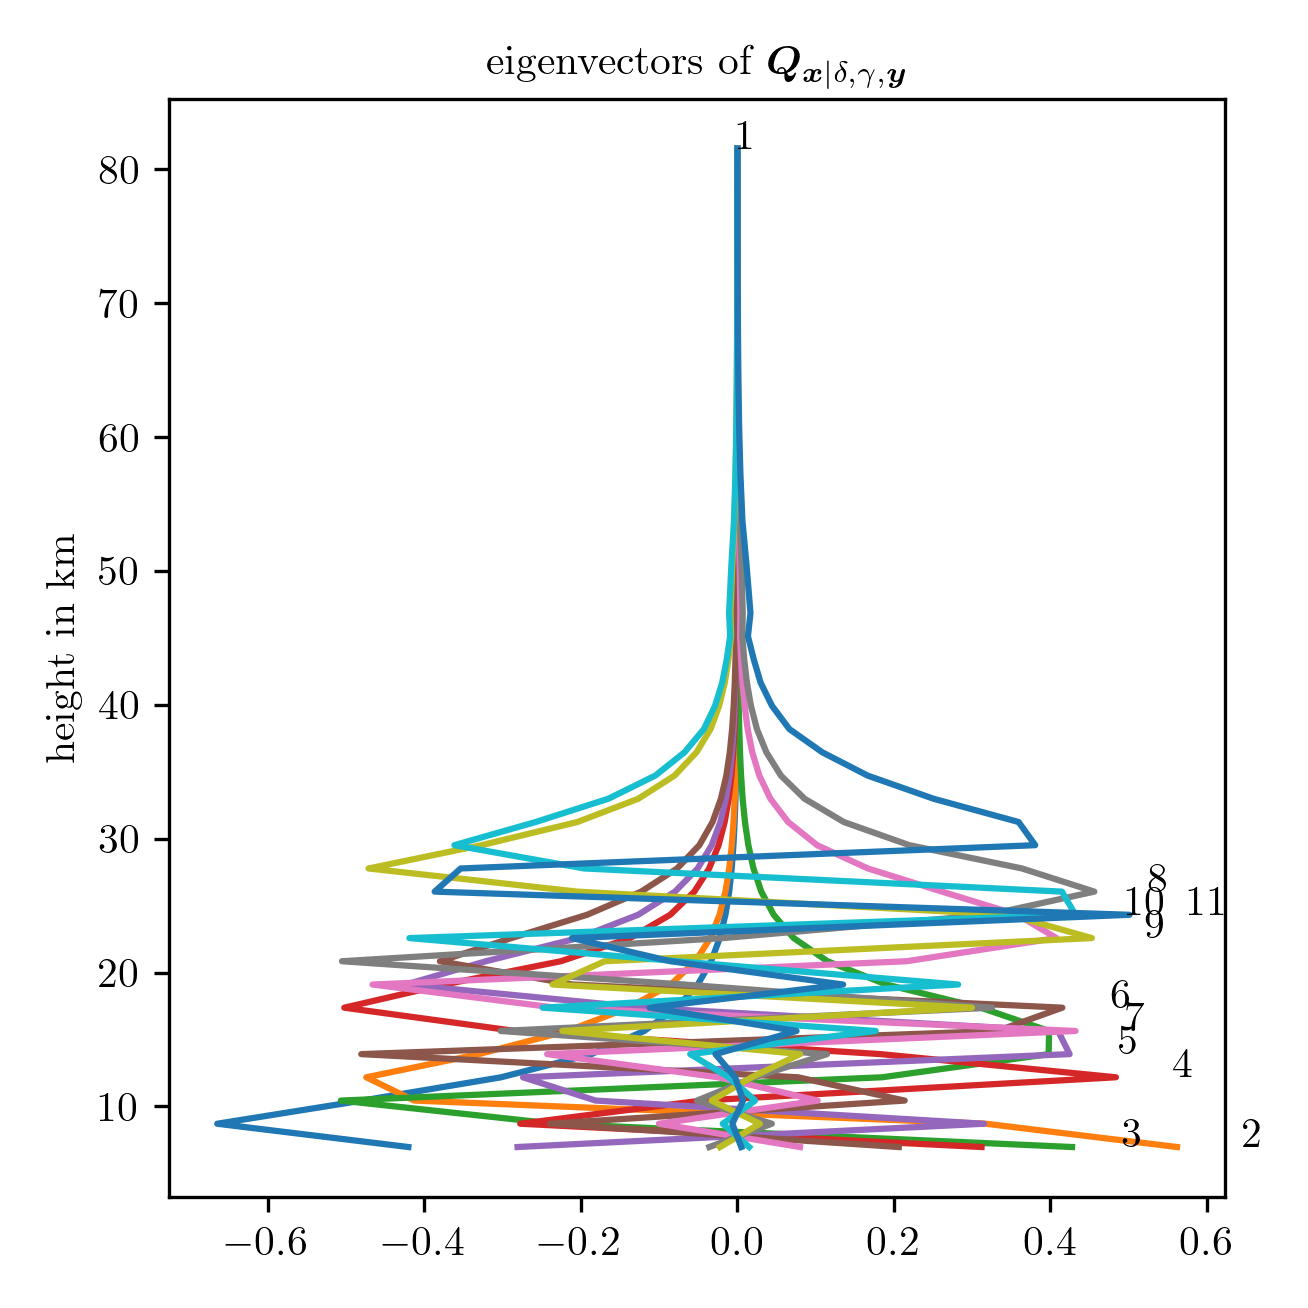
\includegraphics{CovEigVec1.png}
 	\caption[First 11 eigenvectors of conditional precision matrix.]{First 11 eigenvectors corresponding to in size ordered eigenvalues of conditional precision matrix $\bm{Q}_{ \bm{x}|\delta, \gamma, \bm{y}}$.
 	We see that the eigenvectors span structures for heights $\leq 40$.}
 	\label{fig:CovEigVec1}
 \end{figure}
 \begin{figure}[ht!]
 	\centering
 	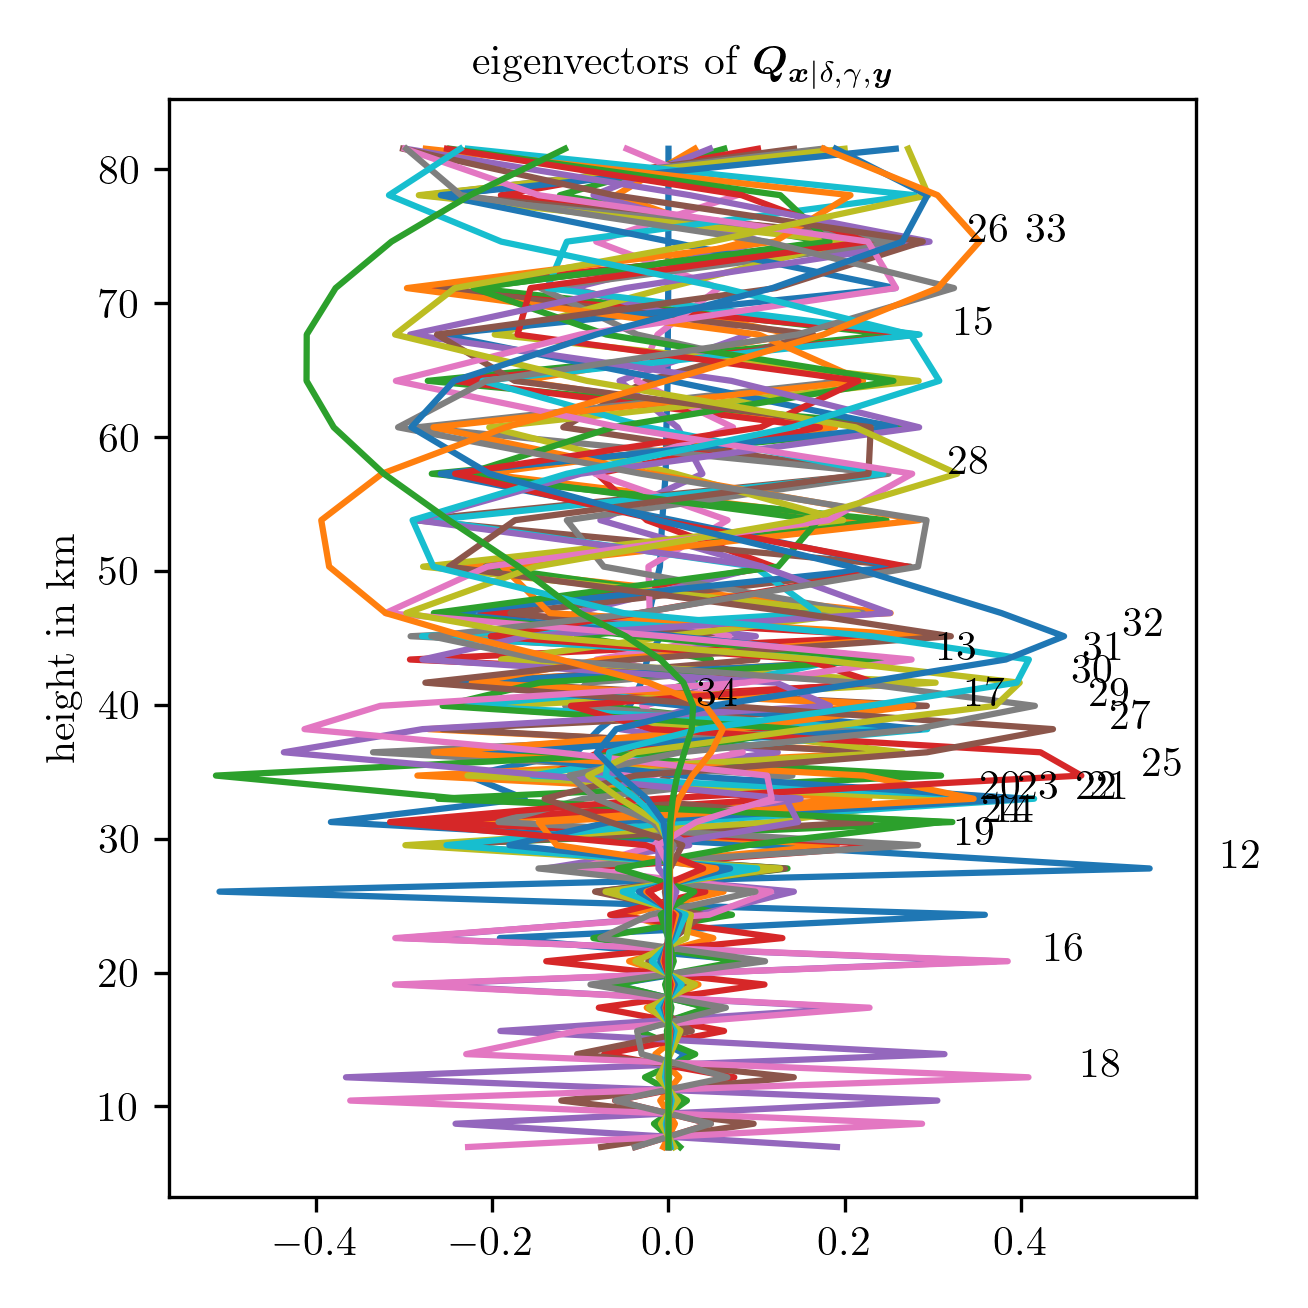
\includegraphics{CovEigVec2.png}
 	\caption[Last 23 eigenvectors of conditional precision matrix.]{Last 23 eigenvectors corresponding to in size ordered eigenvalues of conditional precision matrix $\bm{Q}_{ \bm{x}|\delta, \gamma, \bm{y}}$. The eigenvectors represent structures according to the prior.}
 	\label{fig:CovEigVec2}
 \end{figure}
\clearpage
\section{Pressure and Temperature}

\subsection{Priors}
\begin{figure}[ht!]
	\centering
	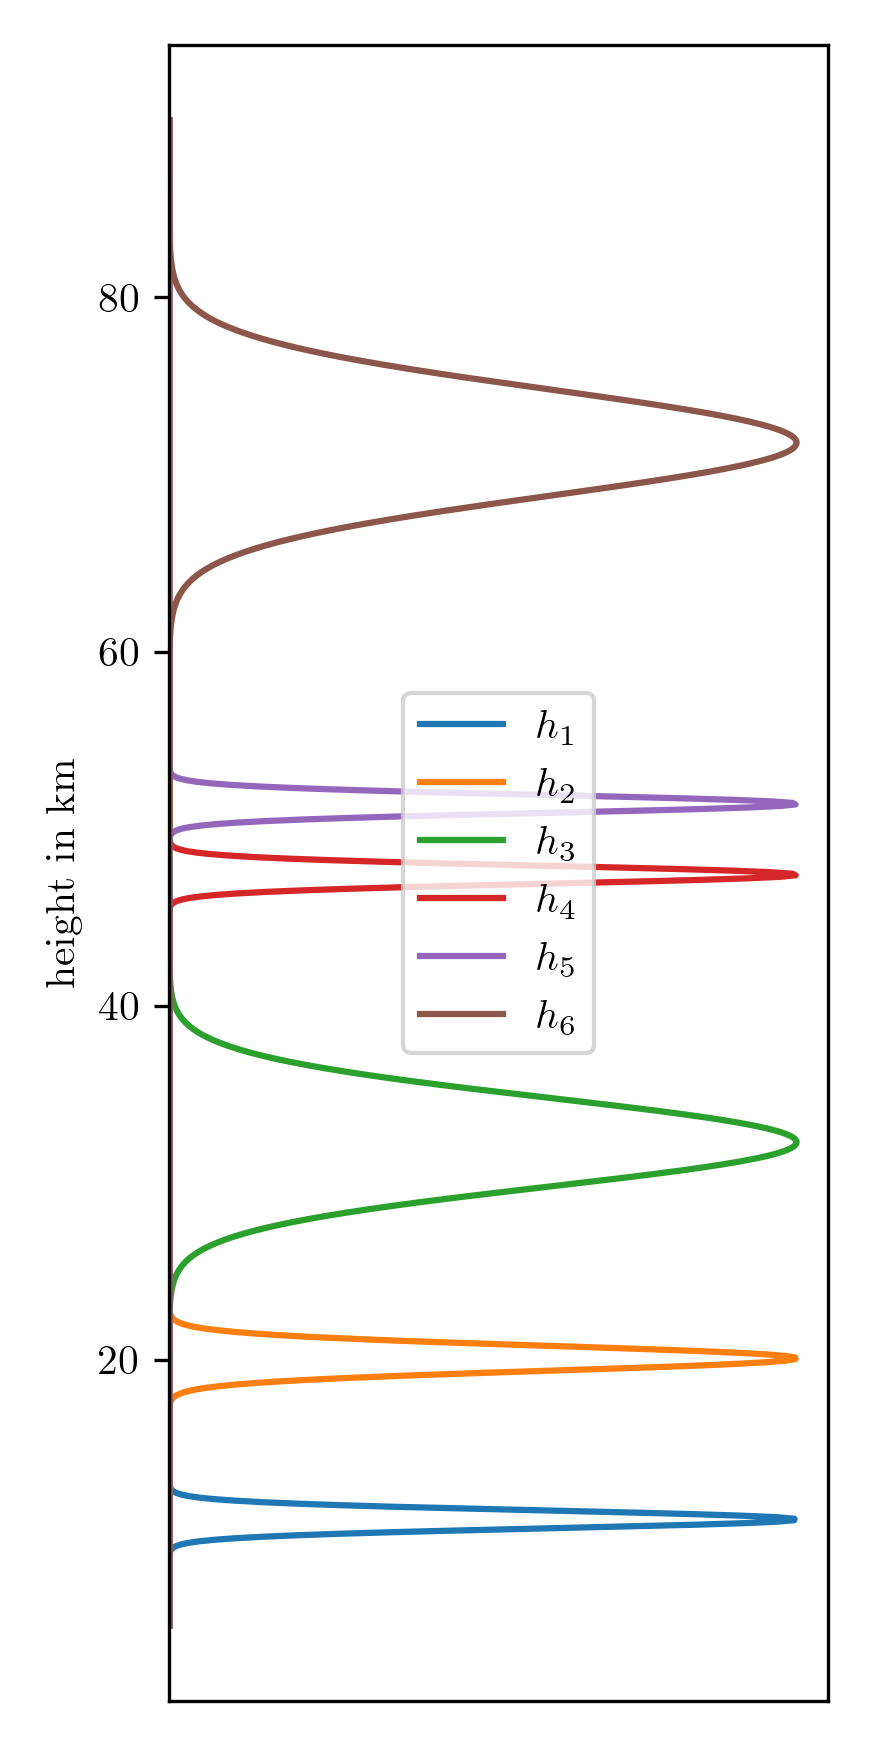
\includegraphics{HeightPriors.png}
	\caption[Prior distributions $\pi(\bm{h_T})$.]{Prior distributions $\pi(\bm{h_T})$, which we choose so that they do not overlap and not conflict with the temperature function in Eq.~\ref{eq:tempFunc}.}
	\label{fig:HeightPriors}
\end{figure} 

\begin{figure}[ht!]
	\centering
	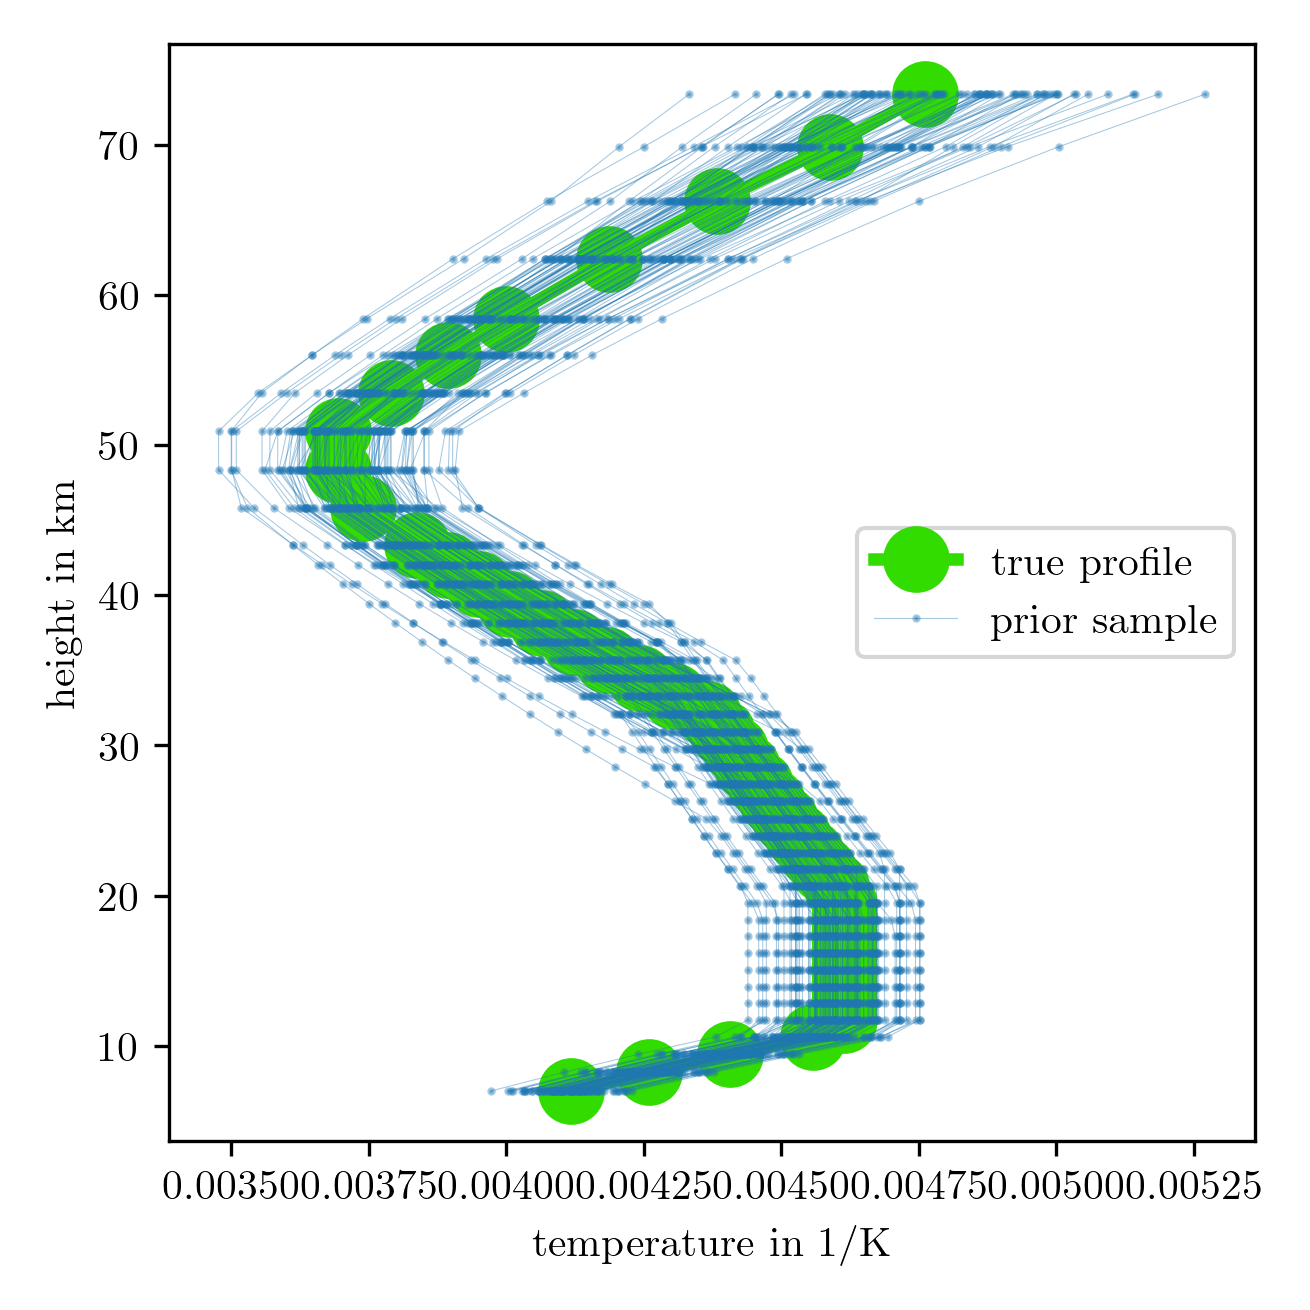
\includegraphics{PriorOverTempPost.png}
	\caption[Prior samples of $1/\bm{T}$]{Prior samples of the inverted temperature profile.}
	\label{fig:OverTempPrior}
\end{figure}
\clearpage
\subsection{T-walk Trace}
\begin{figure}[ht!]
	\centering
	\includegraphics{TraceTwalk.png}
	\caption[T-walk trace]{Output trace of the t-walk on the posterior distribution $\pi(p_0,b,\bm{h_T},\bm{a}| \gamma,\bm{y})$.}
	\label{fig:TraceTwalk}
\end{figure}
\clearpage

\subsection{Integrated Autocorrelation Plots} 
\begin{figure}[ht!]
	\centering
	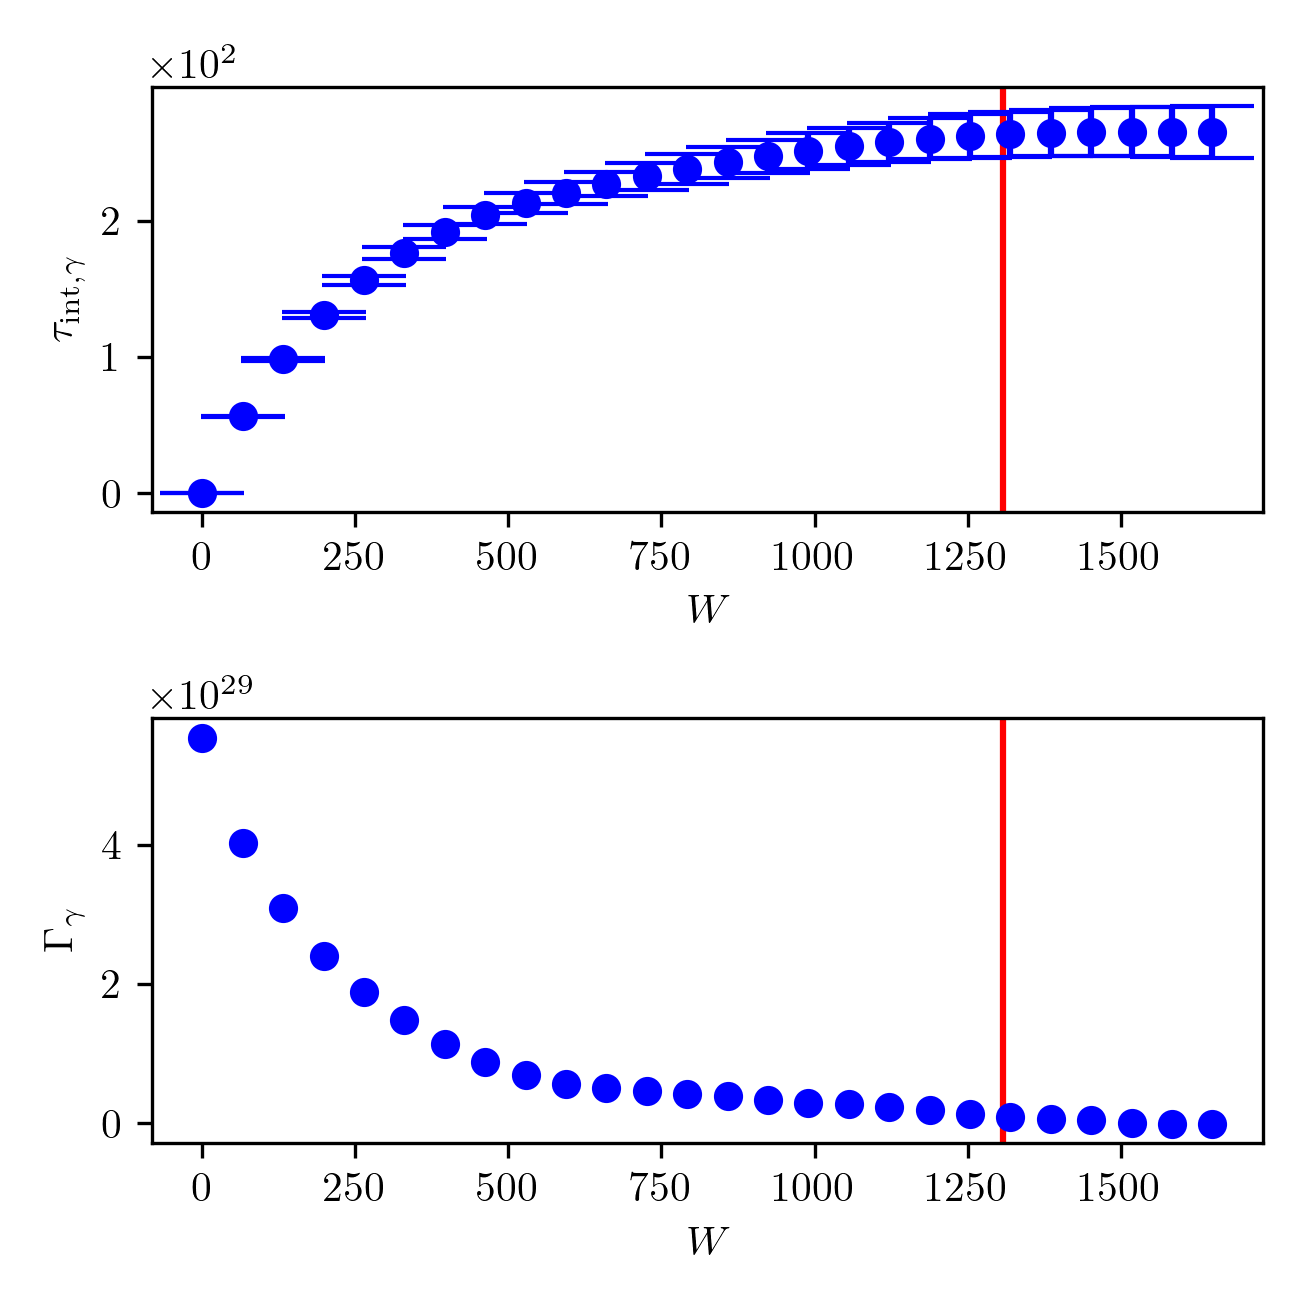
\includegraphics{UwerrTauIntTWalk0.png}
	\caption[IACT and autocorrelation function of samples $\gamma \sim \pi(\cdot|\bm{y})$, for approximated model.]{Provided by \cite{drikHesse}, the IACT $\tau_{\text{int},\gamma }$ at summation windows W and the estimated autocorrelation function $\Gamma_{\gamma }$ at lag $t$ of samples $\gamma  \sim \pi( \cdot| \bm{y})$ from the t-walk for the approximated forward model.}
	\label{fig:TWalkIATC1}
\end{figure}
\begin{figure}[ht!]
	\centering
	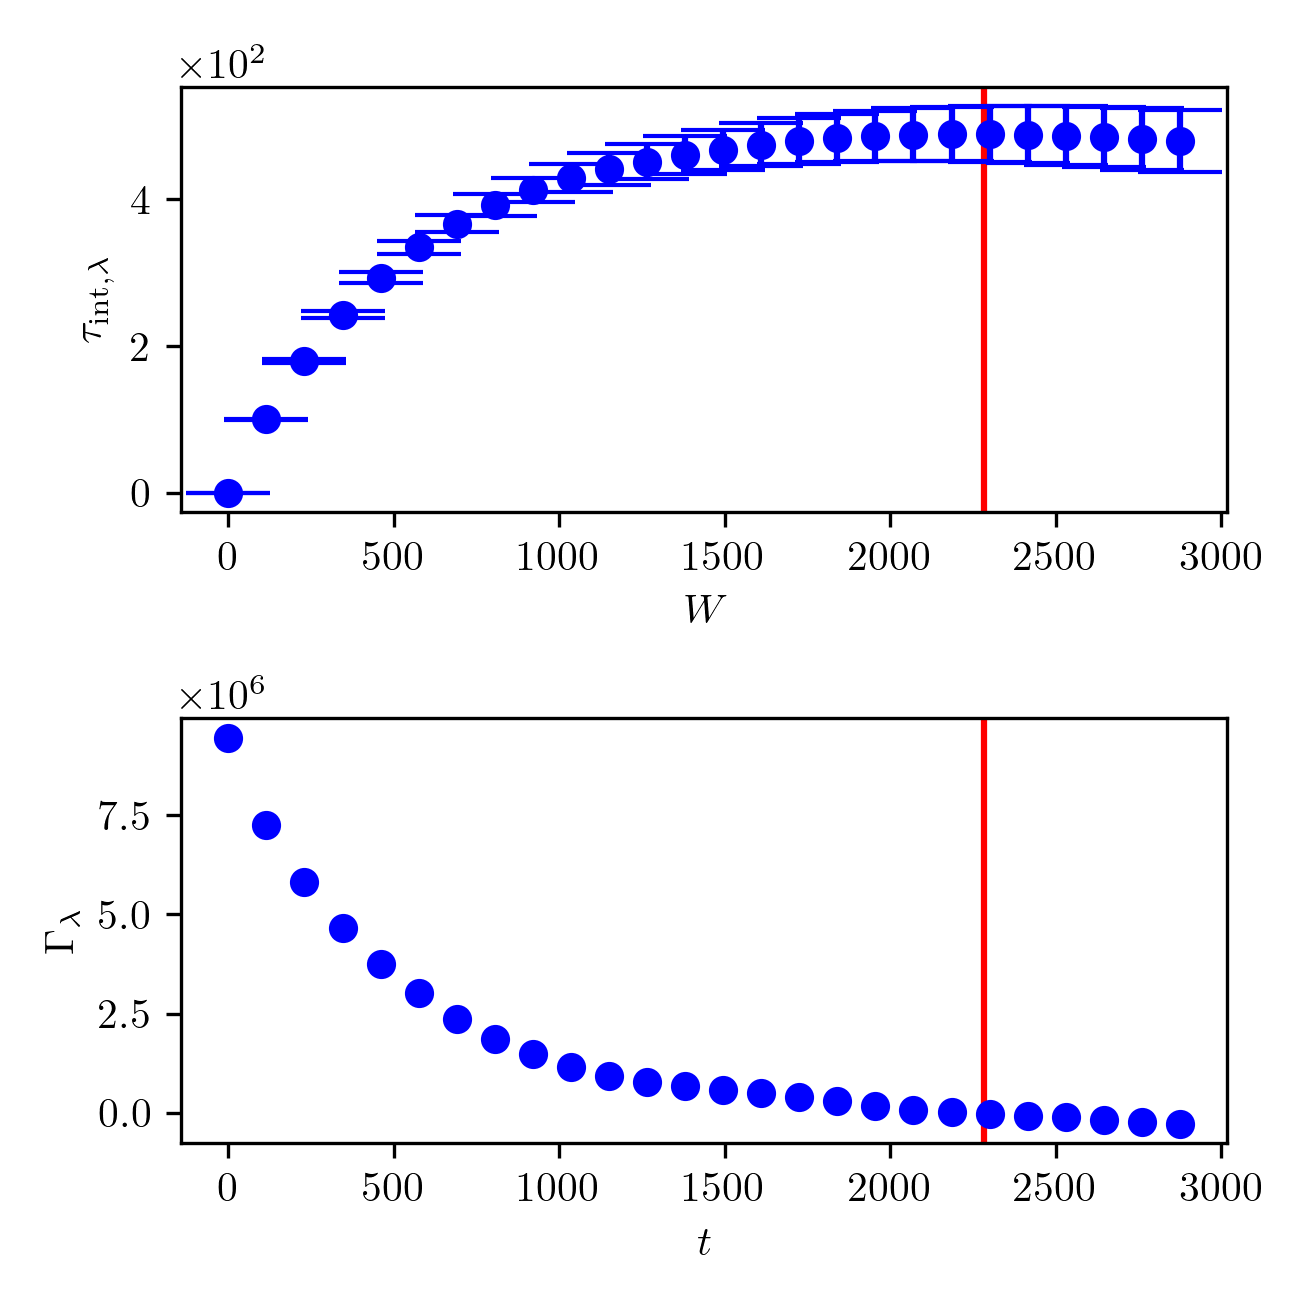
\includegraphics{UwerrTauIntTWalk1.png}
	\caption[IACT and autocorrelation function of samples $\lambda \sim \pi(\cdot|\bm{y})$, for approximated model.]{Provided by \cite{drikHesse}, the IACT $\tau_{\text{int},\lambda}$ at summation windows W and the estimated autocorrelation function $\Gamma_{\lambda}$ at lag $t$ of samples $\lambda \sim \pi( \cdots| \bm{y})$ from the t-walkfor the approximated forward model.}
	\label{fig:TWalkIATC2}
\end{figure}


\begin{figure}[ht!]
	\centering
	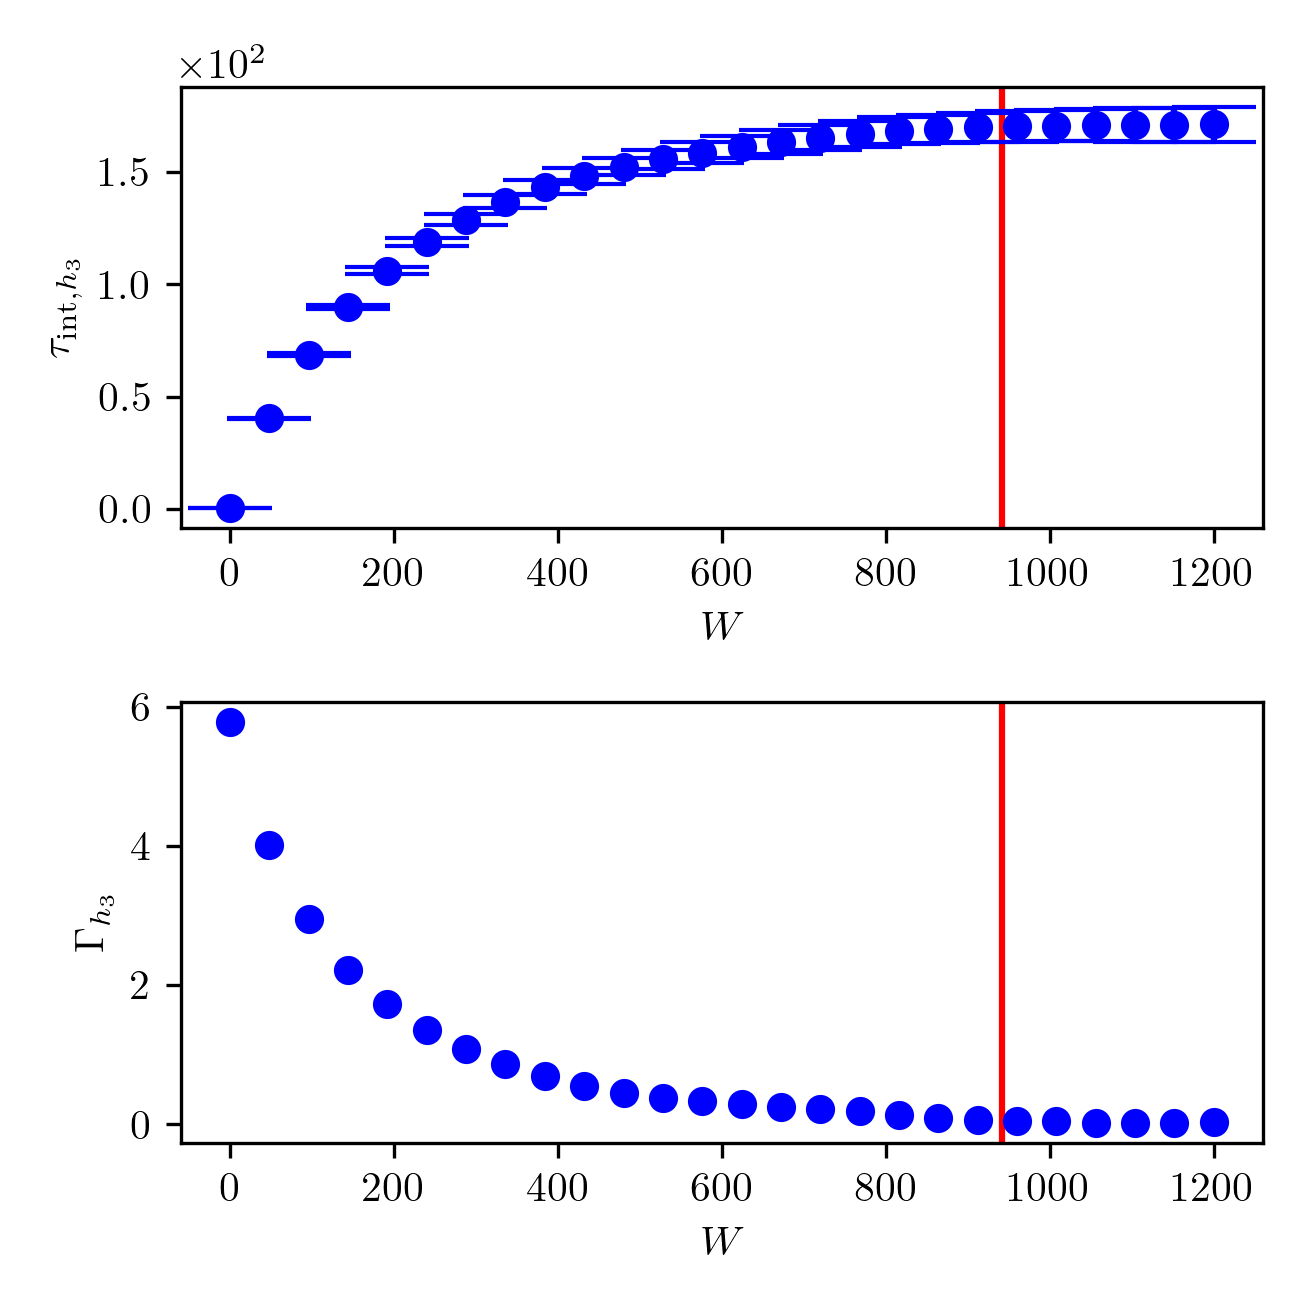
\includegraphics{UwerrTauIntTWalk2.png}
	\caption[IACT and autocorrelation function of samples $b \sim \pi(\cdot|\bm{y})$, for approximated model.]{Provided by \cite{drikHesse}, the IACT $\tau_{\text{int},b}$ at summation windows W and the estimated autocorrelation function $\Gamma_{b}$ at lag $t$ of samples $b \sim \pi( \cdot| \bm{y})$ from the t-walk for the approximated forward model.}
	\label{fig:TWalkIATC3}
\end{figure}


\begin{figure}[ht!]
	\centering
	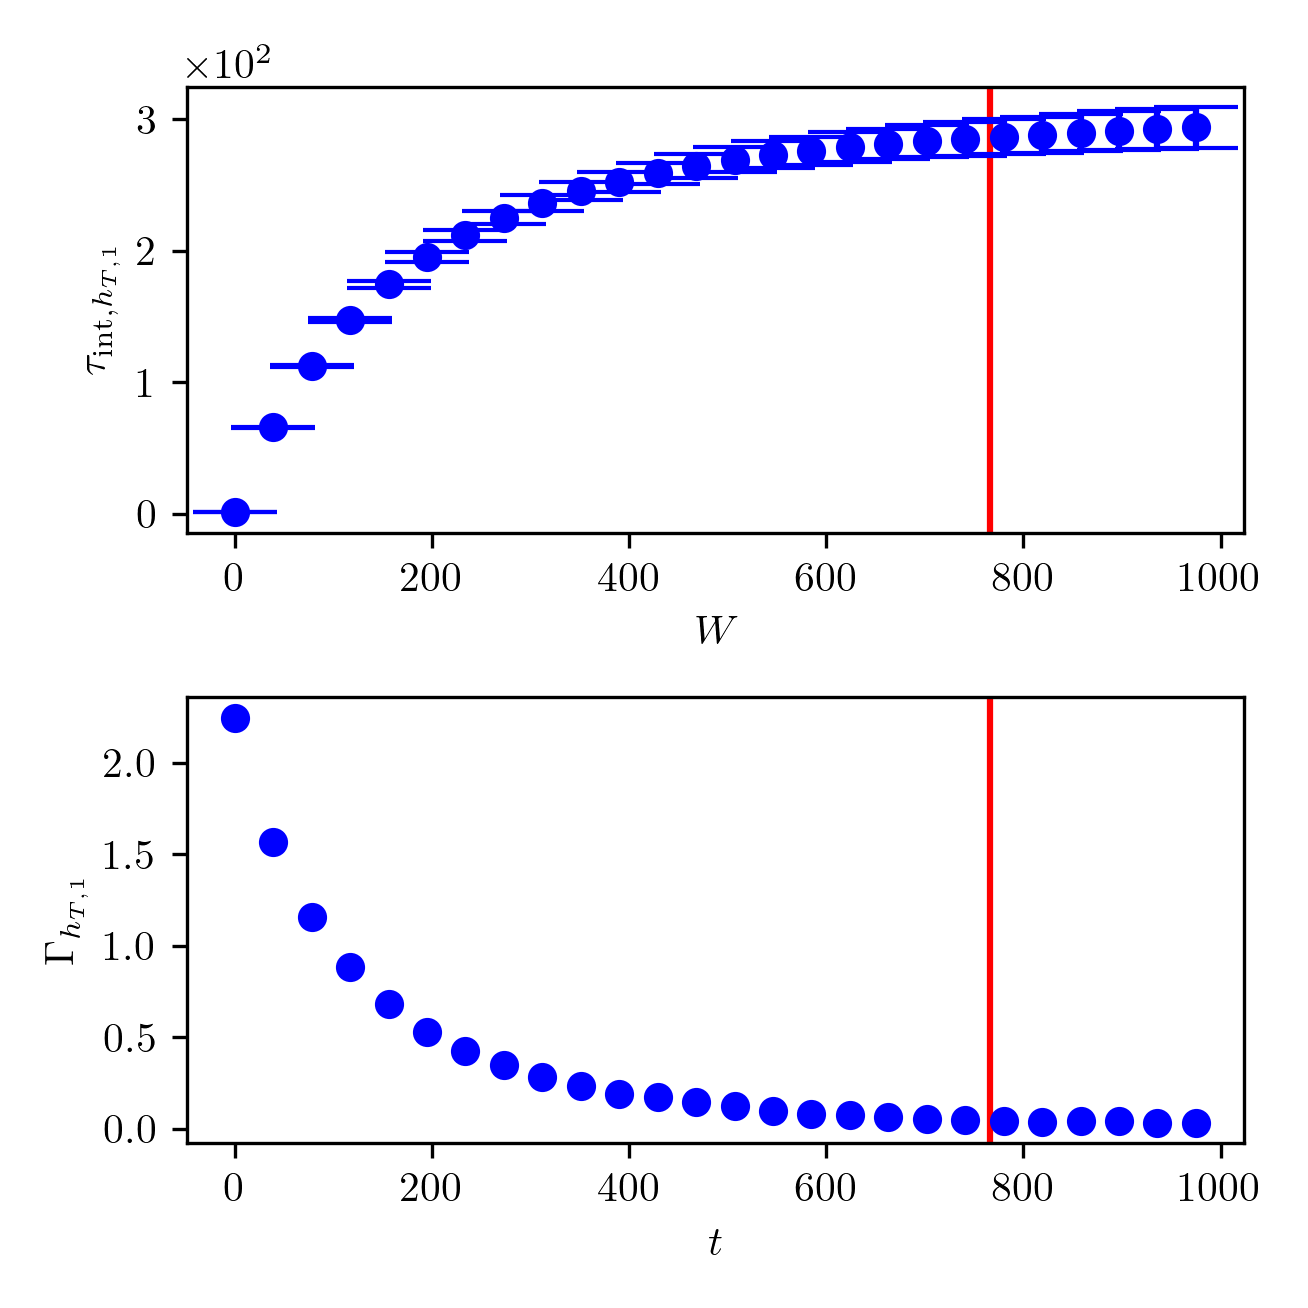
\includegraphics{UwerrTauIntTWalk3.png}
	\caption[IACT and autocorrelation function of samples $h_{T,1} \sim \pi(\cdot|\bm{y})$, for approximated model.]{Provided by \cite{drikHesse}, the IACT $\tau_{\text{int},h_{T,1}}$ at summation windows W and the estimated autocorrelation function $\Gamma_{h_{T,1}}$ at lag $t$ of samples $h_{T,1} \sim \pi( \cdot| \bm{y})$ from the t-walk for the approximated forward model.}
	\label{fig:TWalkIATC4}
\end{figure}


\begin{figure}[ht!]
	\centering
	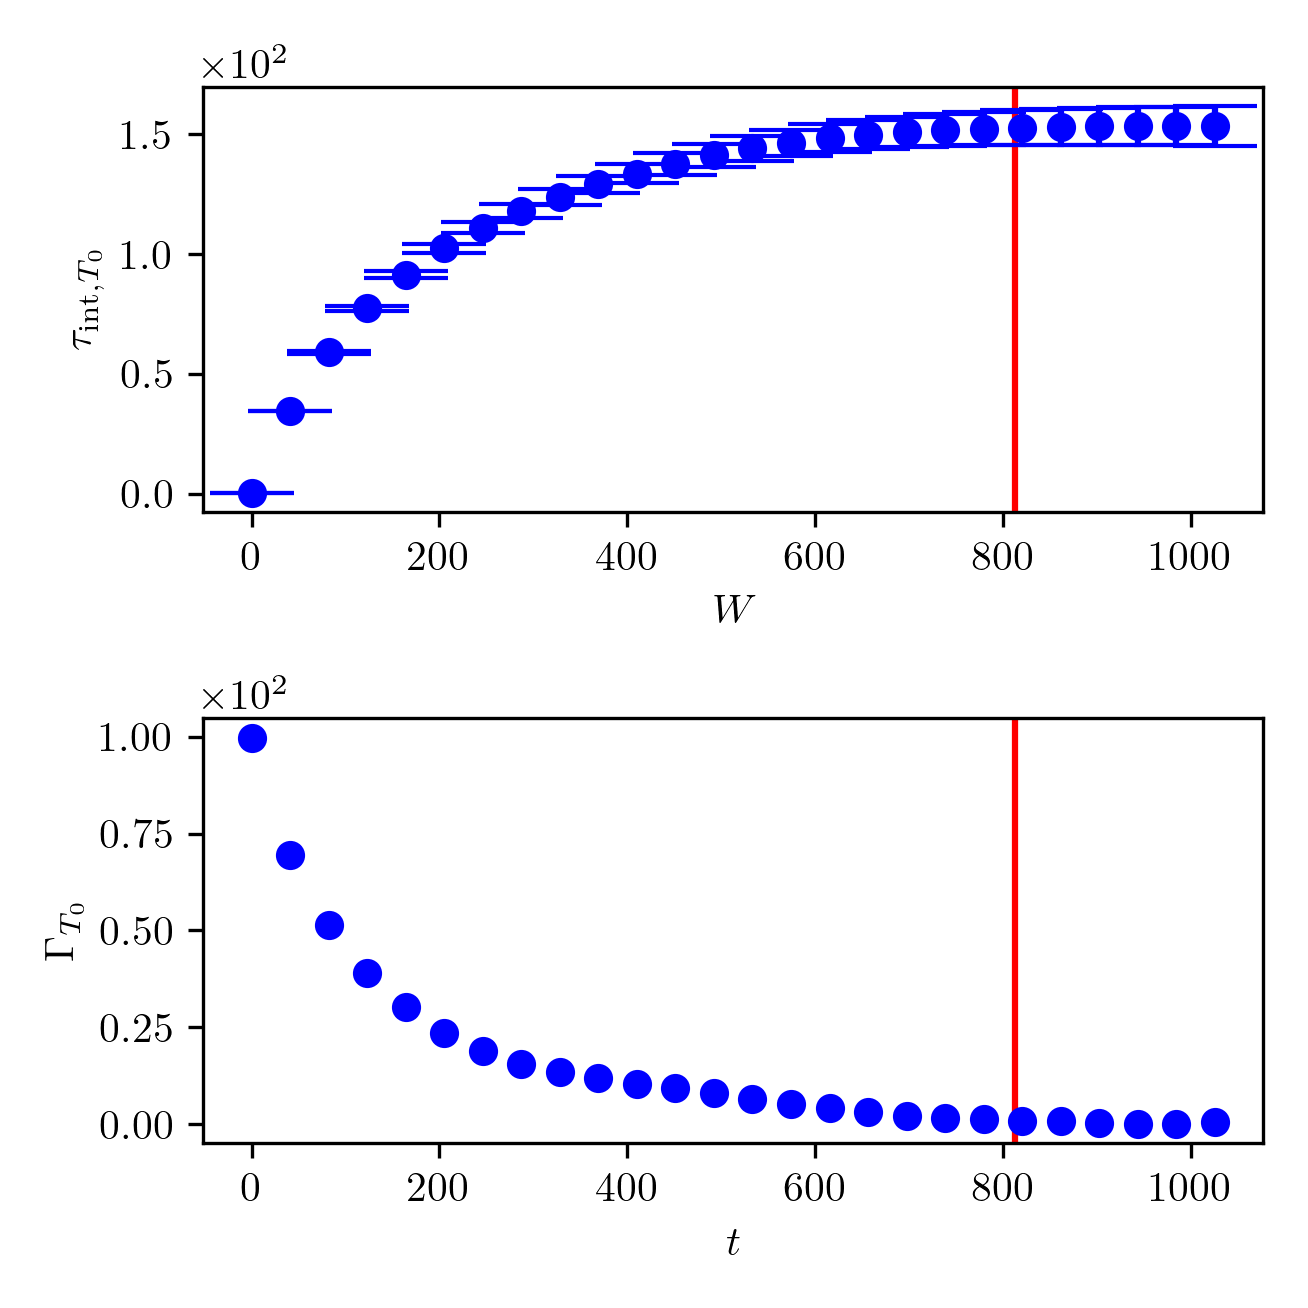
\includegraphics{UwerrTauIntTWalk4.png}
	\caption[IACT and autocorrelation function of samples $T_0  \sim \pi(\cdot|\bm{y})$, for approximated model.]{Provided by \cite{drikHesse}, the IACT $\tau_{\text{int},T_0}$ at summation windows W and the estimated autocorrelation function $\Gamma_{T_0}$ at lag $t$ of samples $T_0 \sim \pi( \cdot| \bm{y})$ from the t-walk for the approximated forward model.}
	\label{fig:TWalkIATC5}
\end{figure}


\begin{figure}[ht!]
	\centering
	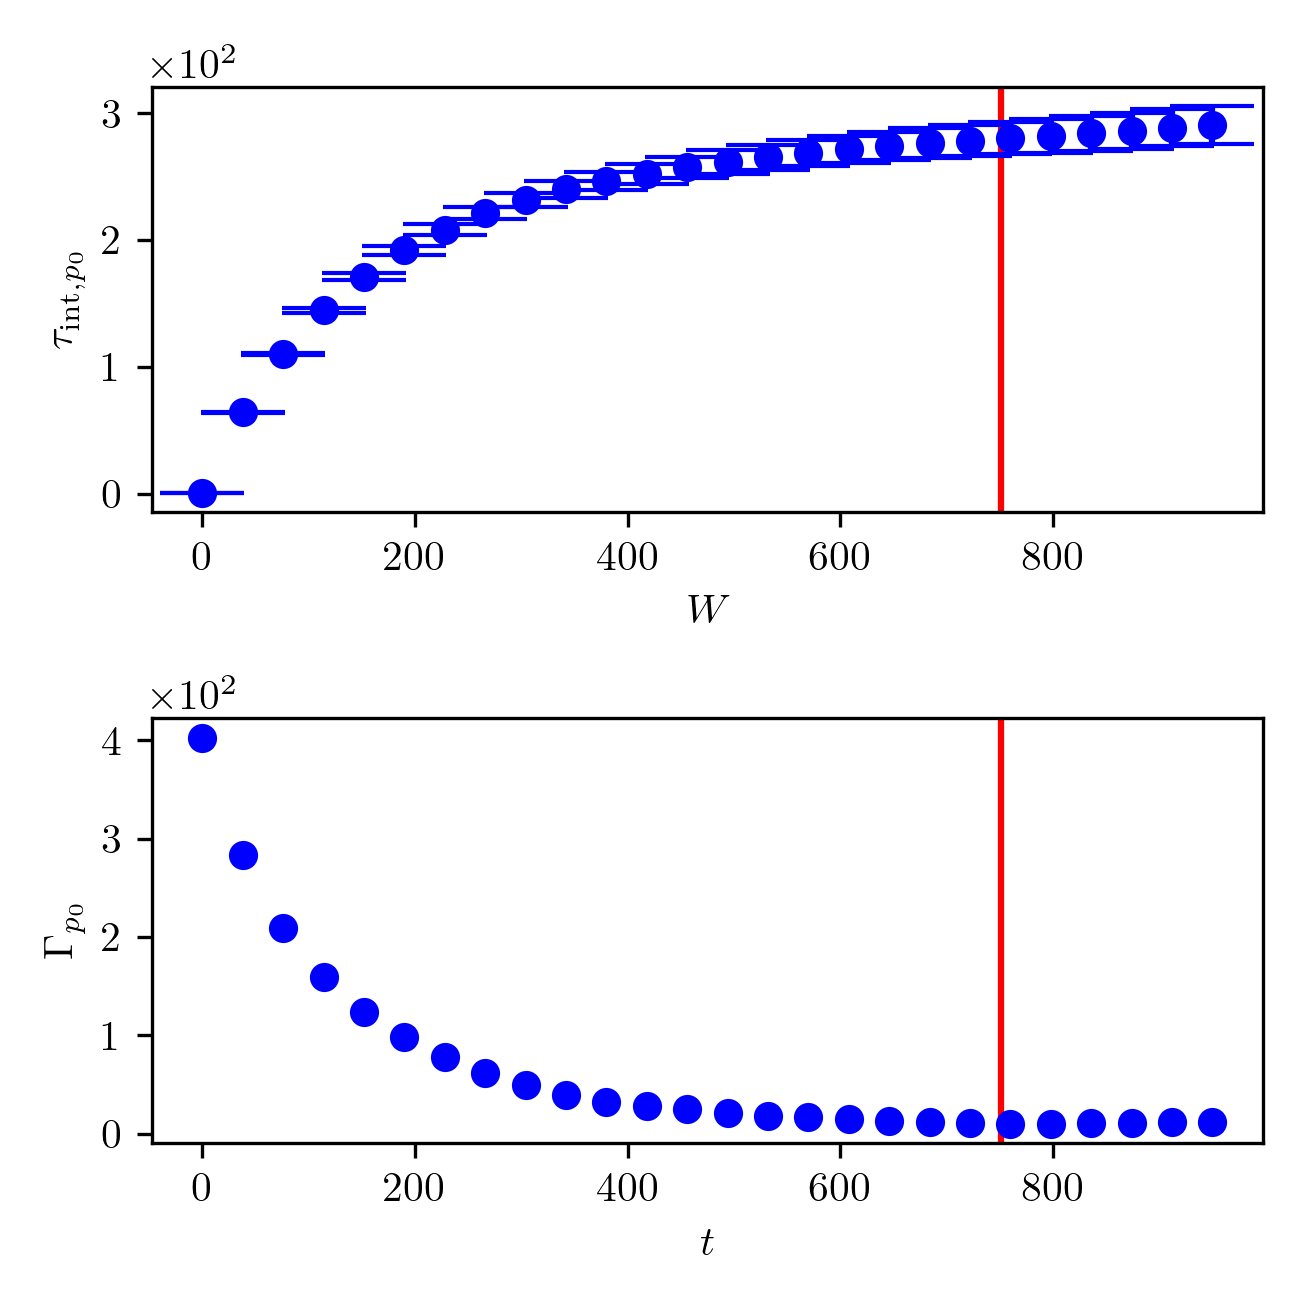
\includegraphics{UwerrTauIntTWalk5.png}
	\caption[IACT and autocorrelation function of samples $p_0 \sim \pi(\cdot|\bm{y})$, for approximated model.]{Provided by \cite{drikHesse}, the IACT $\tau_{\text{int},p_0}$ at summation windows W and the estimated autocorrelation function $\Gamma_{p_0}$ at lag $t$ of samples $p_0 \sim \pi( \cdot| \bm{y})$ from the t-walk for the approximated forward model.}
	\label{fig:TWalkIATC6}
\end{figure}


\begin{figure}[ht!]
	\centering
	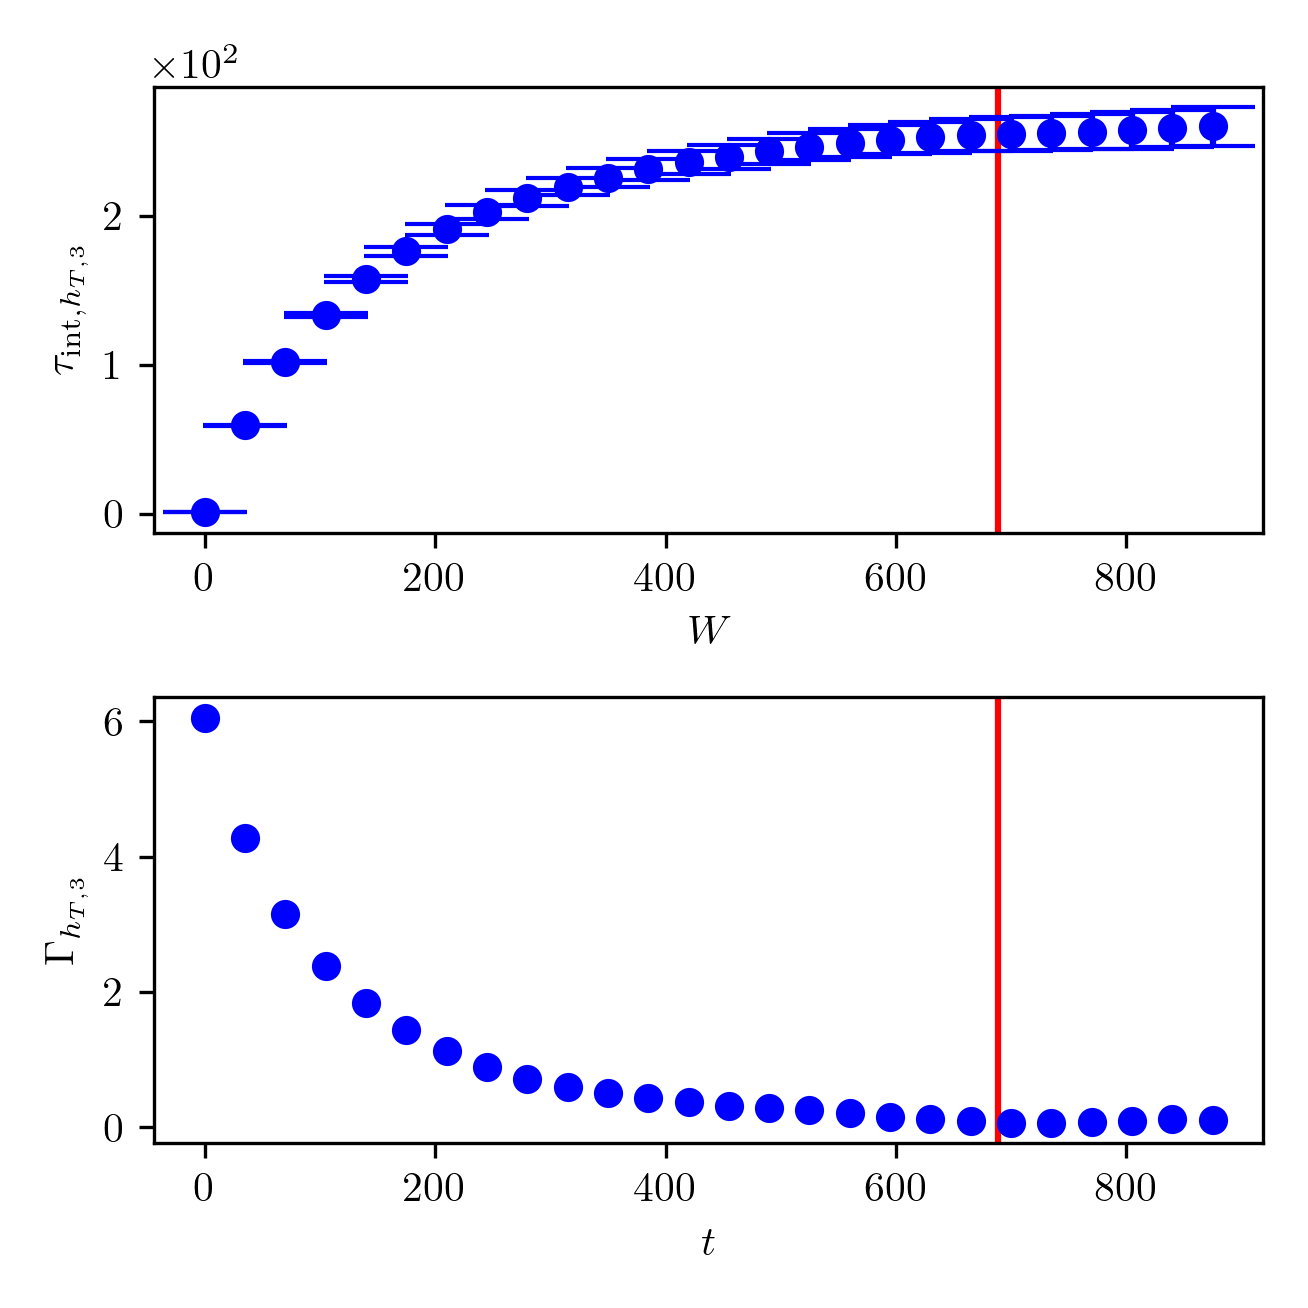
\includegraphics{UwerrTauIntTWalk6.png}
	\caption[IACT and autocorrelation function of samples $h_{T,3} \sim \pi(\cdot|\bm{y})$, for approximated model.]{Provided by \cite{drikHesse}, the IACT $\tau_{\text{int},h_{T,3}}$ at summation windows W and the estimated autocorrelation function $\Gamma_{h_{T,3}}$ at lag $t$ of samples $h_{T,3} \sim \pi( \cdot| \bm{y})$ from the t-walk for the approximated forward model.}
	\label{fig:TWalkIATC7}
\end{figure}

\begin{figure}[ht!]
	\centering
	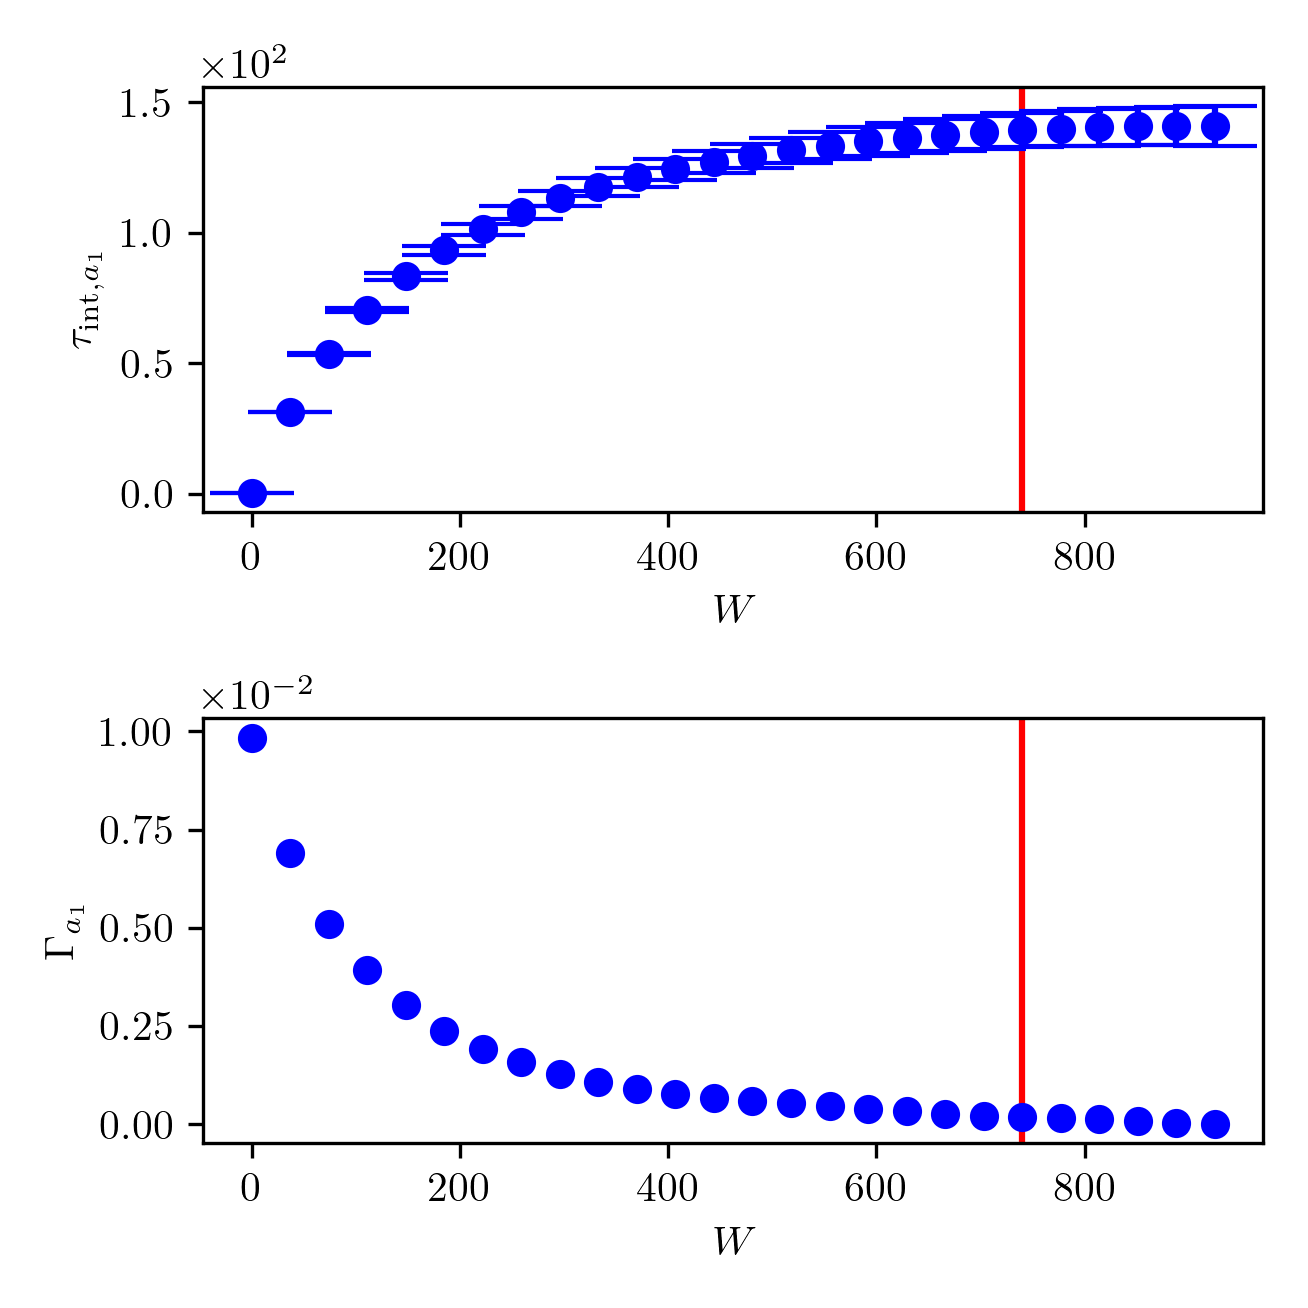
\includegraphics{UwerrTauIntTWalk7.png}
	\caption[IACT and autocorrelation function of samples $a_1 \sim \pi(\cdot|\bm{y})$, for approximated model.]{Provided by \cite{drikHesse}, the IACT $\tau_{\text{int},a_1}$ at summation windows W and the estimated autocorrelation function $\Gamma_{a_1}$ at lag $t$ of samples $a_1 \sim \pi( \cdot| \bm{y})$ from the t-walk for the approximated forward model.}
	\label{fig:TWalkIATC8}
\end{figure}


\begin{figure}[ht!]
	\centering
	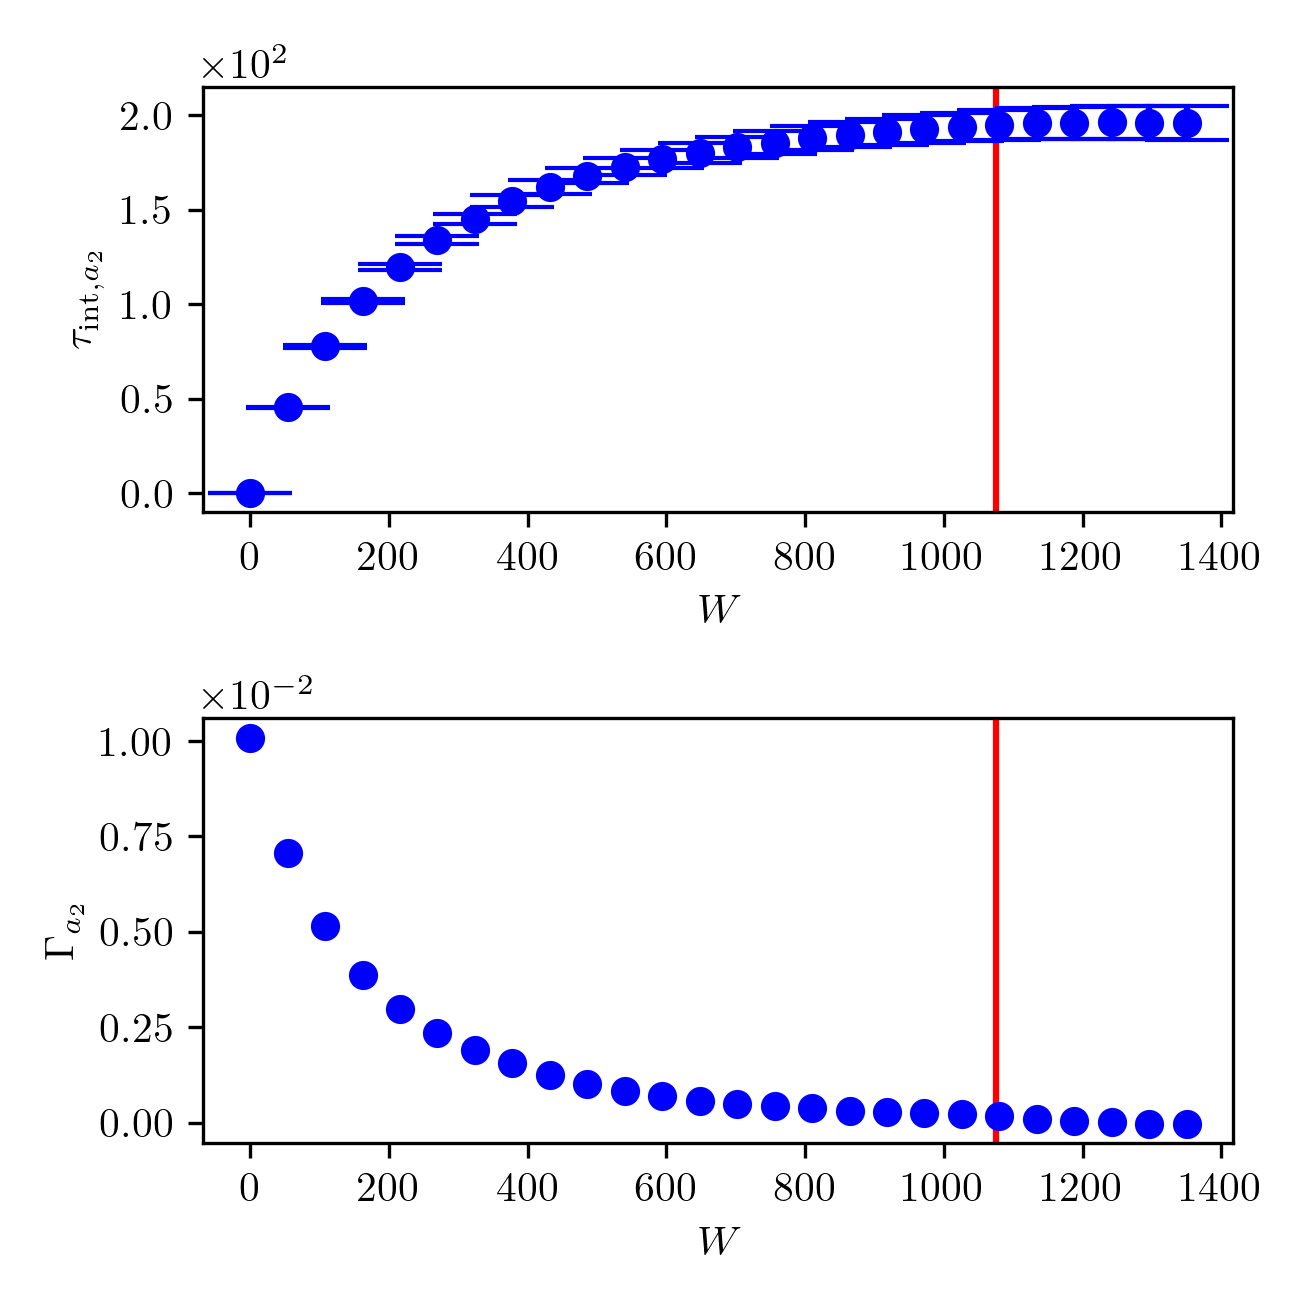
\includegraphics{UwerrTauIntTWalk8.png}
	\caption[IACT and autocorrelation function of samples $h_{T,2} \sim \pi(\cdot|\bm{y})$, for approximated model.]{Provided by \cite{drikHesse}, the IACT $\tau_{\text{int},h_{T,2}}$ at summation windows W and the estimated autocorrelation function $\Gamma_{h_{T,2}}$ at lag $t$ of samples $h_{T,2} \sim \pi( \cdots | \bm{y})$ from the t-walk for the approximated forward model.}
	\label{fig:TWalkIATC9}
\end{figure}


\begin{figure}[ht!]
	\centering
	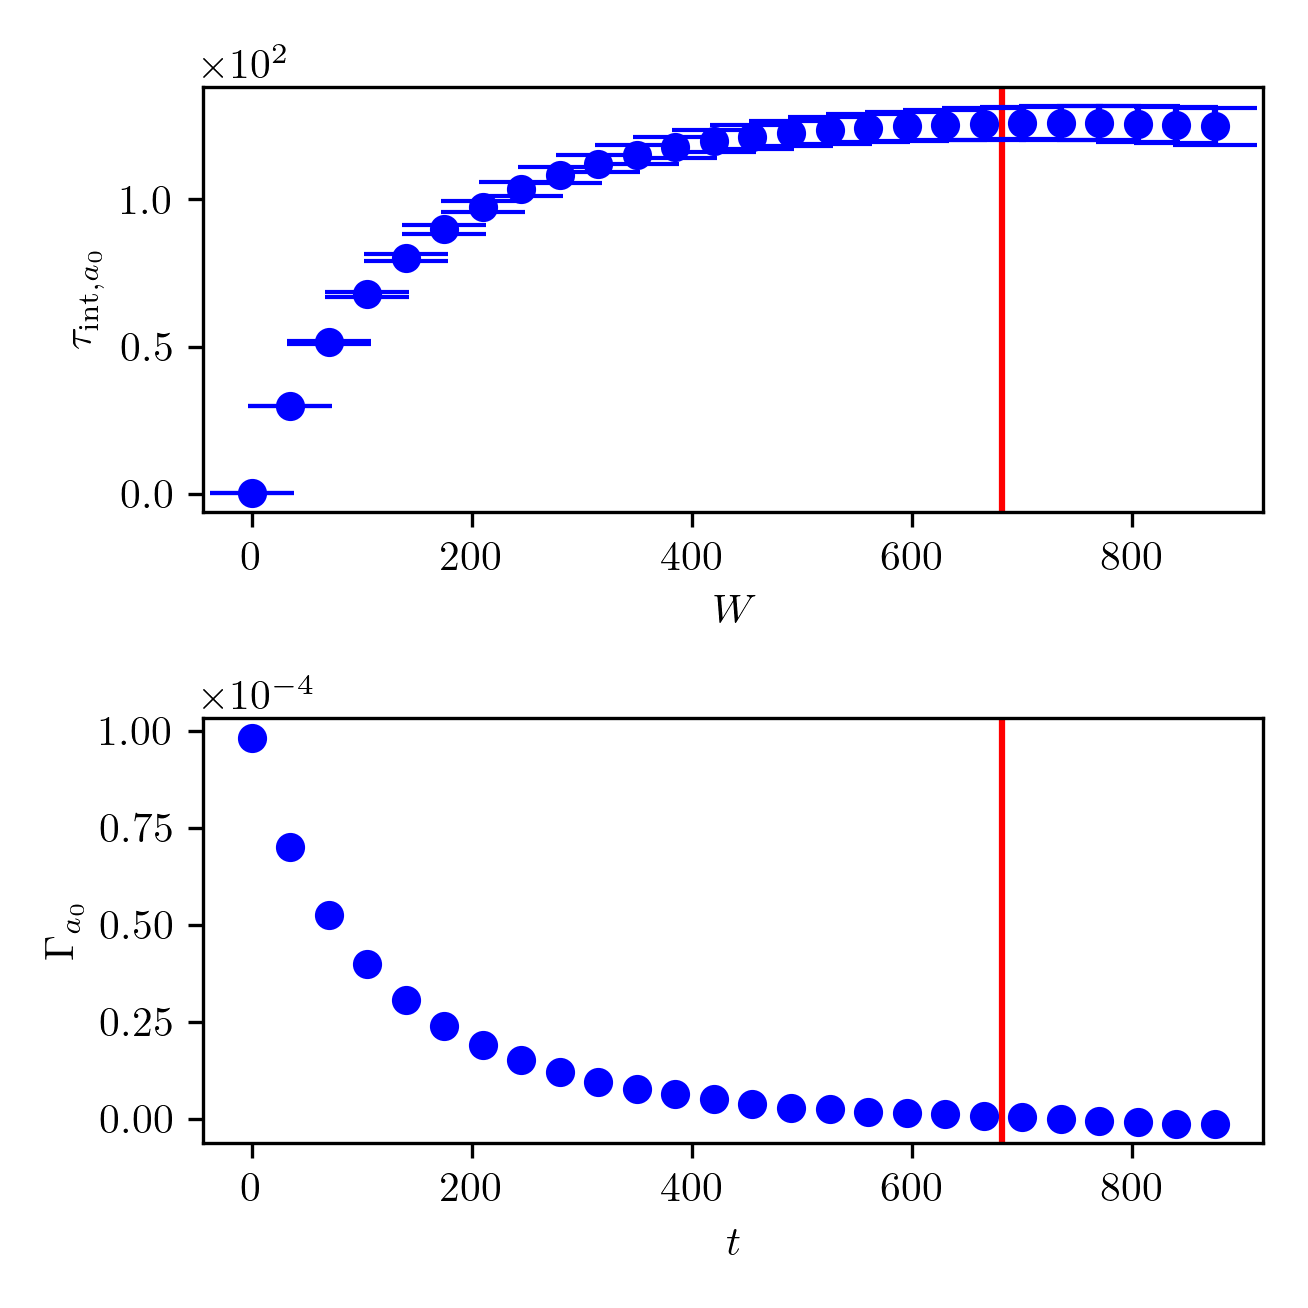
\includegraphics{UwerrTauIntTWalk9.png}
	\caption[IACT and autocorrelation function of samples $a_0 \sim \pi(\cdot|\bm{y})$, for approximated model.]{Provided by \cite{drikHesse}, the IACT $\tau_{\text{int},a_0}$ at summation windows W and the estimated autocorrelation function $\Gamma_{a_0}$ at lag $t$ of samples $a_0 \sim \pi( \cdot| \bm{y})$ from the t-walk for the approximated forward model.}
\end{figure}

\begin{figure}[ht!]
	\centering
	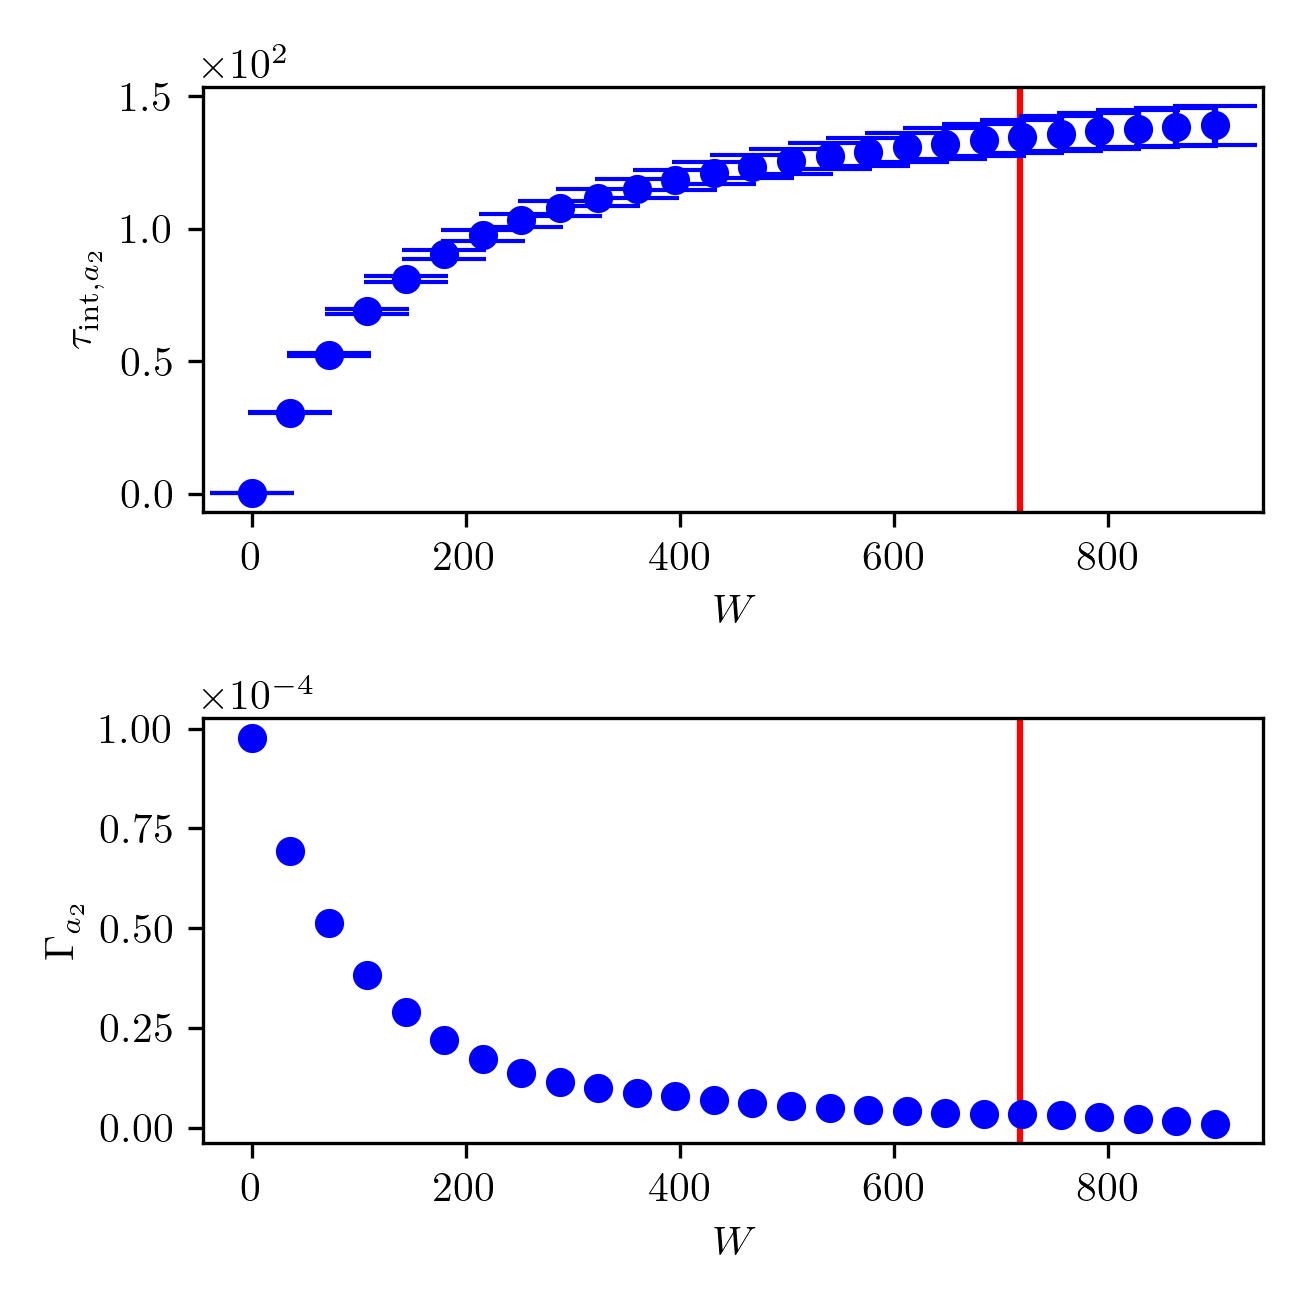
\includegraphics{UwerrTauIntTWalk10.png}
	\caption[IACT and autocorrelation function of samples $a_2 \sim \pi(\cdot|\bm{y})$, for approximated model.]{Provided by \cite{drikHesse}, the IACT $\tau_{\text{int},a_2}$ at summation windows W and the estimated autocorrelation function $\Gamma_{a_2}$ at lag $t$ of samples $a_2 \sim \pi( \cdot | \bm{y})$ from the t-walk for the approximated forward model.}
	\label{fig:TWalkIATC11}
\end{figure}


\begin{figure}[ht!]
	\centering
	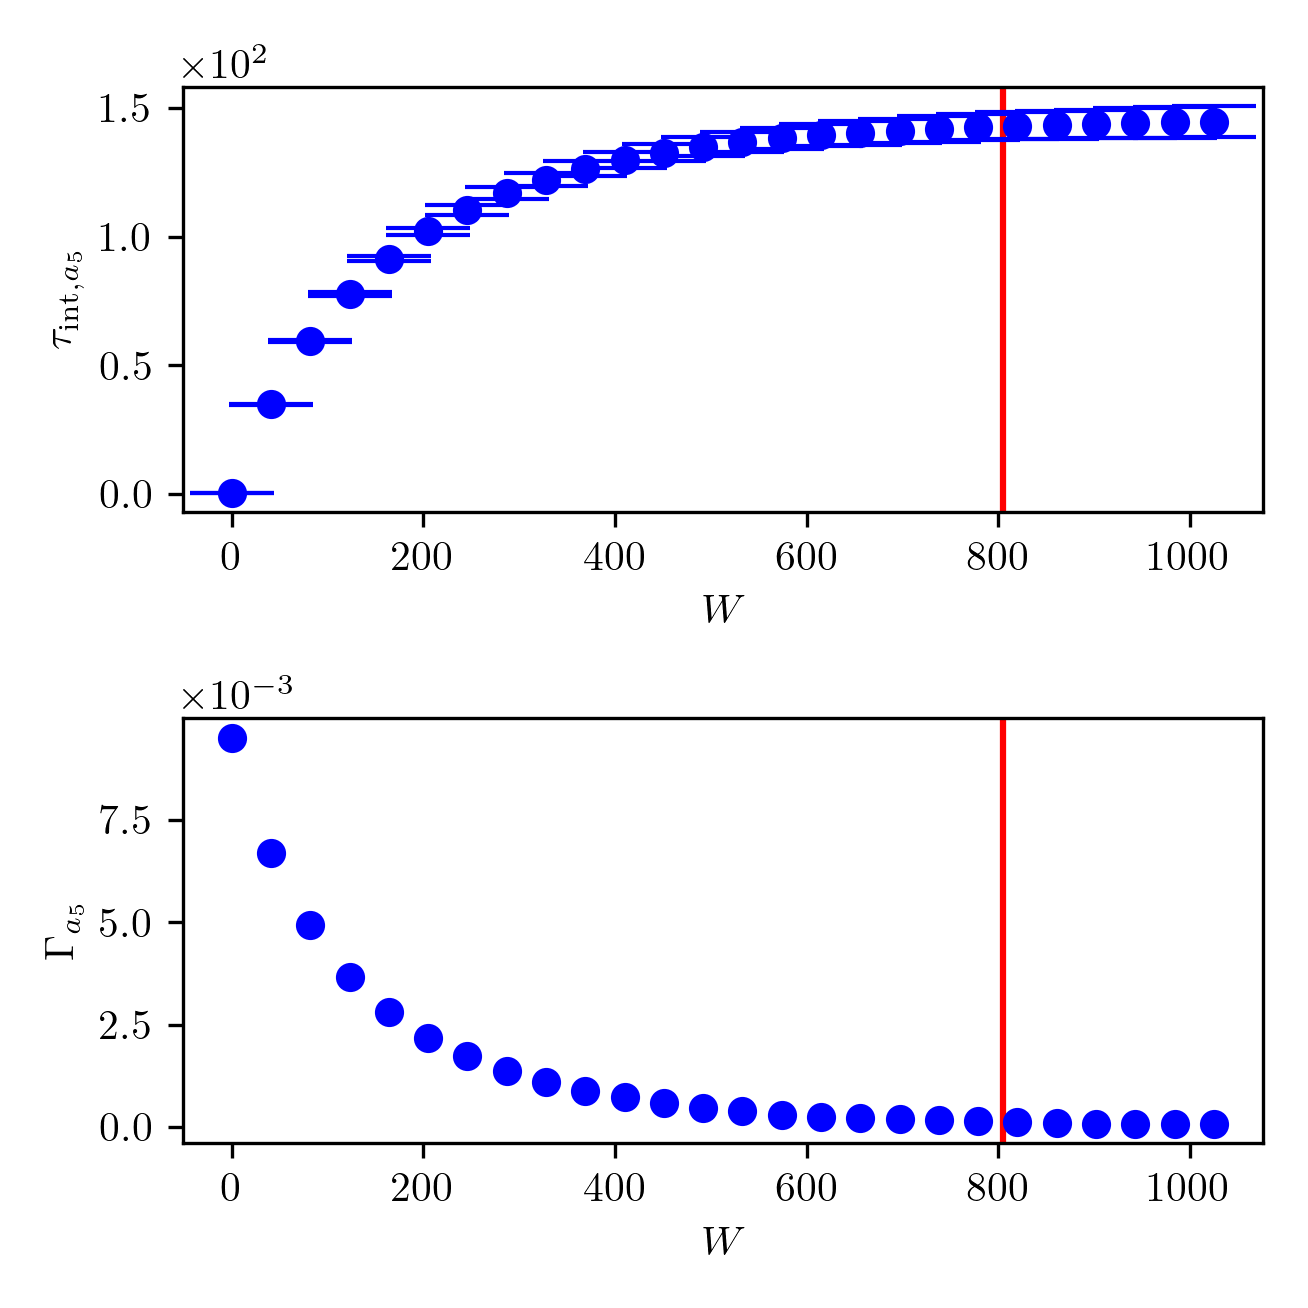
\includegraphics{UwerrTauIntTWalk11.png}
	\caption[IACT and autocorrelation function of samples $a_3 \sim \pi(\cdot|\bm{y})$, for approximated model.]{Provided by \cite{drikHesse}, the IACT $\tau_{\text{int},a_3}$ at summation windows W and the estimated autocorrelation function $\Gamma_{a_3}$ at lag $t$ of samples $a_3 \sim \pi( \cdot| \bm{y})$ from the t-walk for the approximated forward model.}
	\label{fig:TWalkIATC12}
\end{figure}
\begin{figure}[ht!]
	\centering
	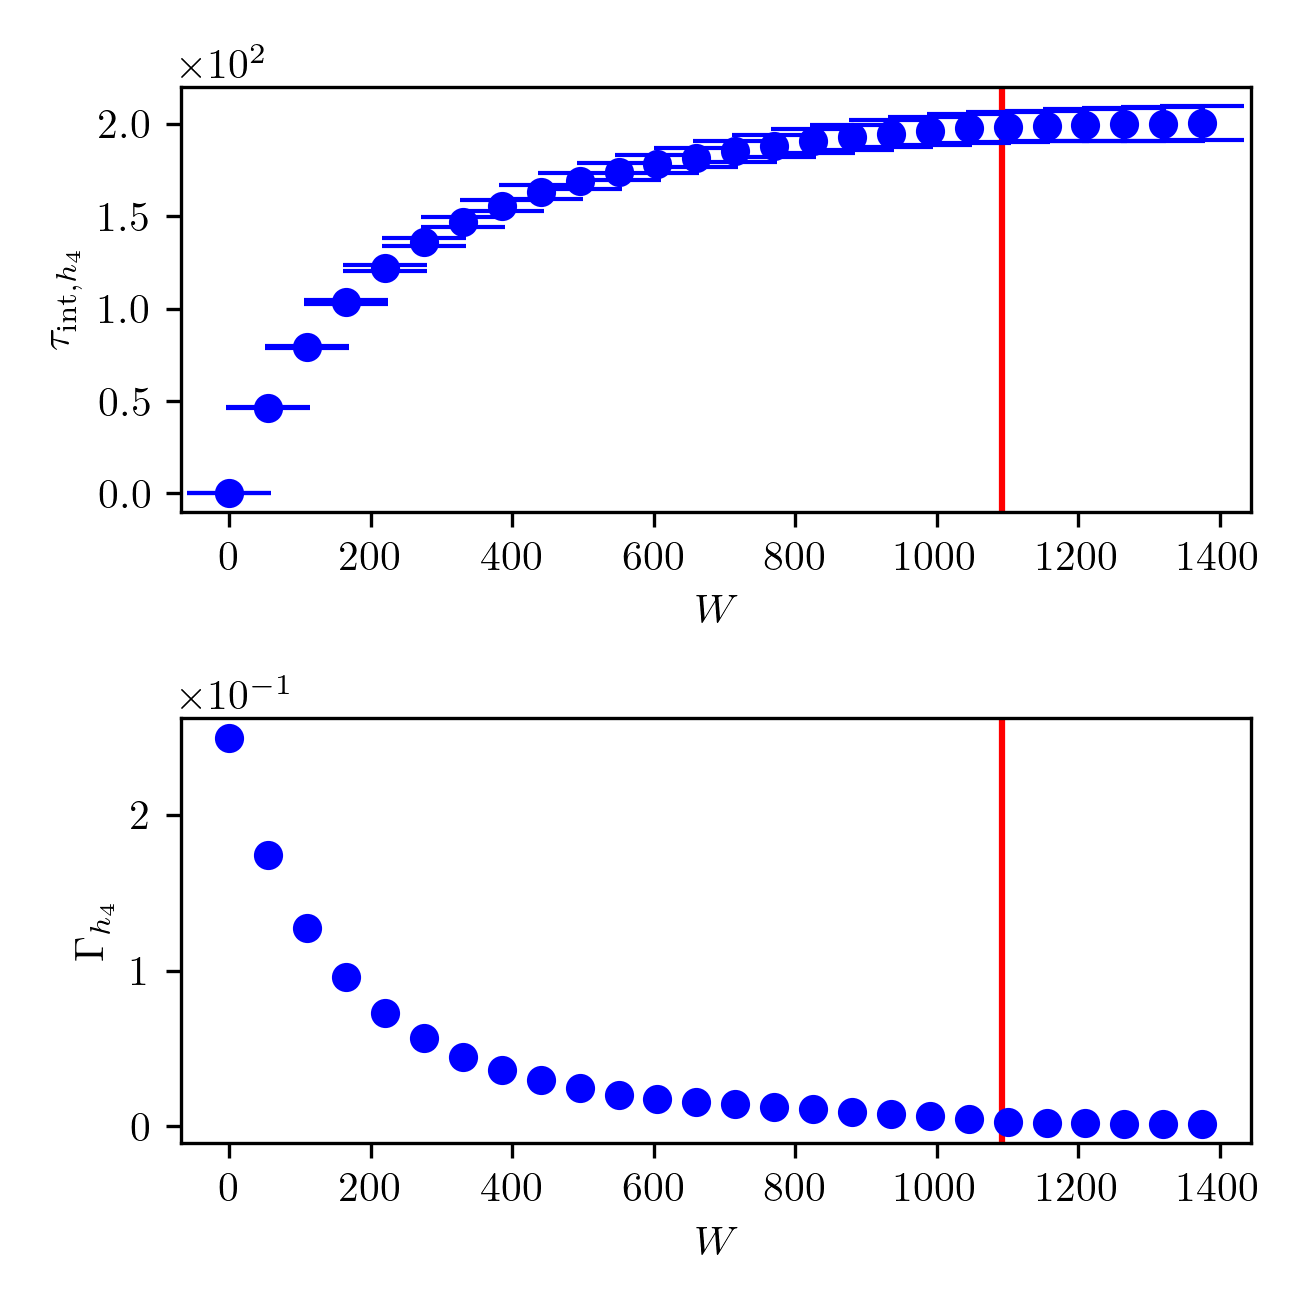
\includegraphics{UwerrTauIntTWalk12.png}
	\caption[IACT and autocorrelation function of samples $h_{T,4} \sim \pi(\cdot|\bm{y})$, for approximated model.]{Provided by \cite{drikHesse}, the IACT $\tau_{\text{int},h_{T,4}}$ at summation windows W and the estimated autocorrelation function $\Gamma_{h_{T,4}}$ at lag $t$ of samples $h_{T,4} \sim \pi( \cdot| \bm{y})$ from the t-walk for the approximated forward model.}
	\label{fig:TWalkIATC13}
\end{figure}
\begin{figure}[ht!]
	\centering
	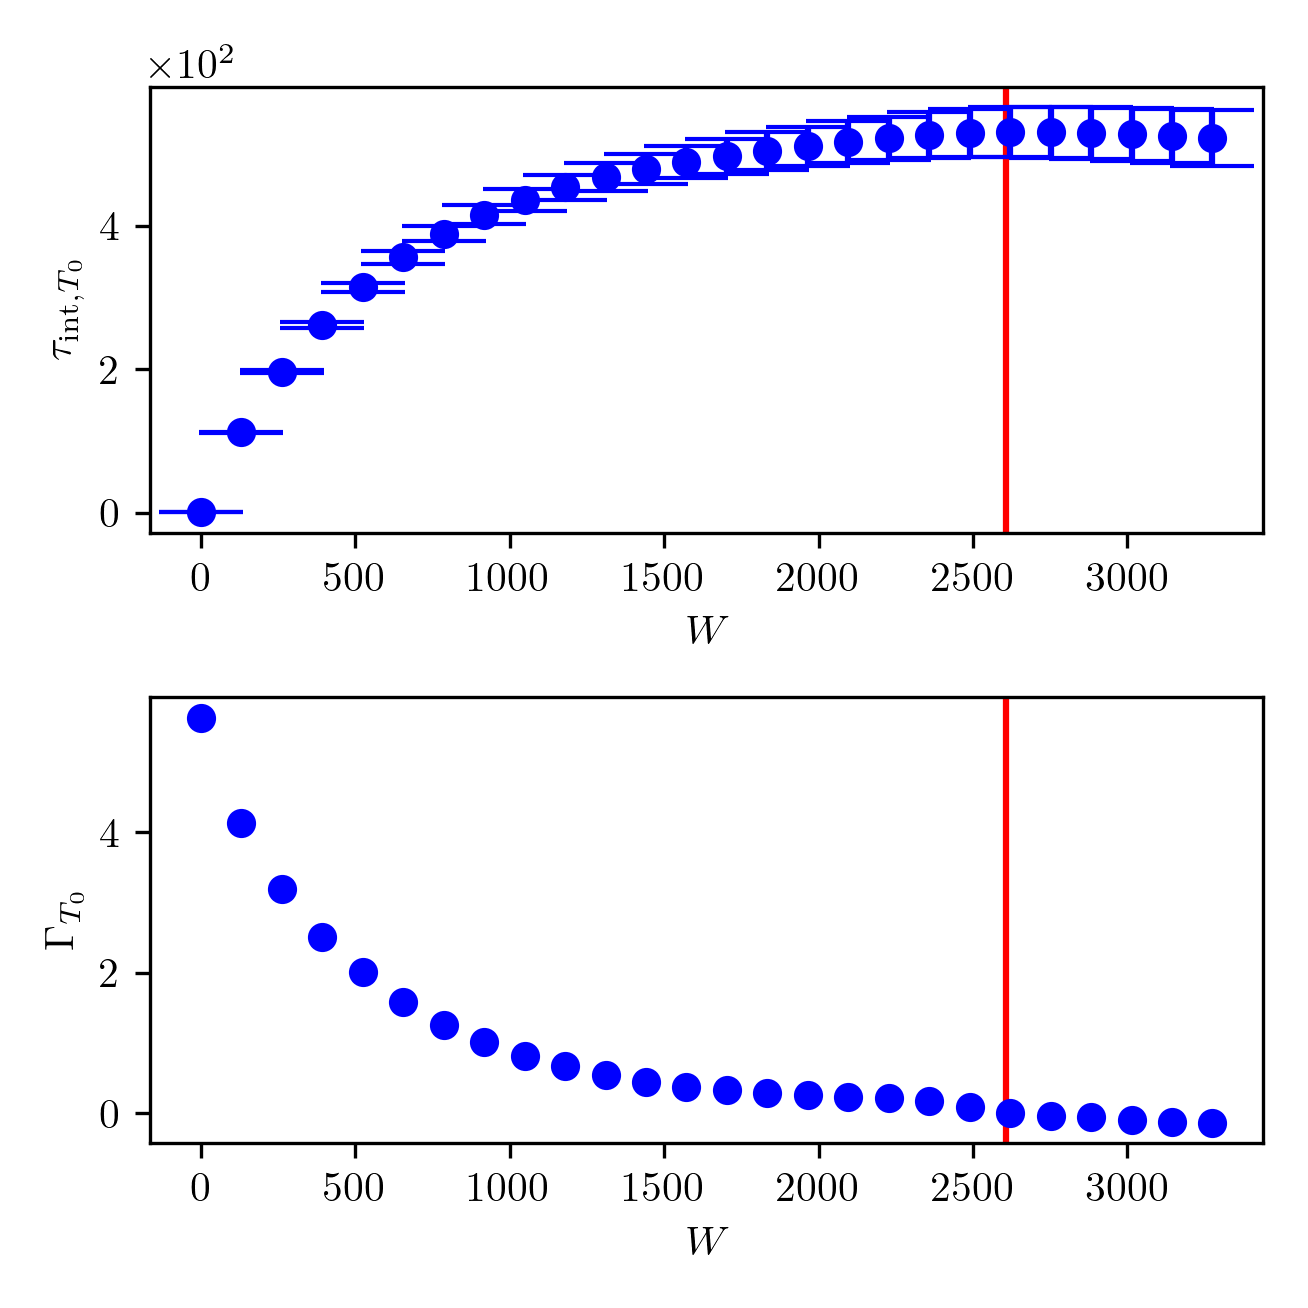
\includegraphics{UwerrTauIntTWalk13.png}
	\caption[IACT and autocorrelation function of samples $a_4 \sim \pi(\cdot|\bm{y})$, for approximated model.]{Provided by \cite{drikHesse}, the IACT $\tau_{\text{int},a_4}$ at summation windows W and the estimated autocorrelation function $\Gamma_{a_4}$ at lag $t$ of samples $a_4 \sim \pi( \cdot| \bm{y})$ from the t-walk for the approximated forward model.}
	\label{fig:TWalkIATC14}
\end{figure}
\begin{figure}[ht!]
	\centering
	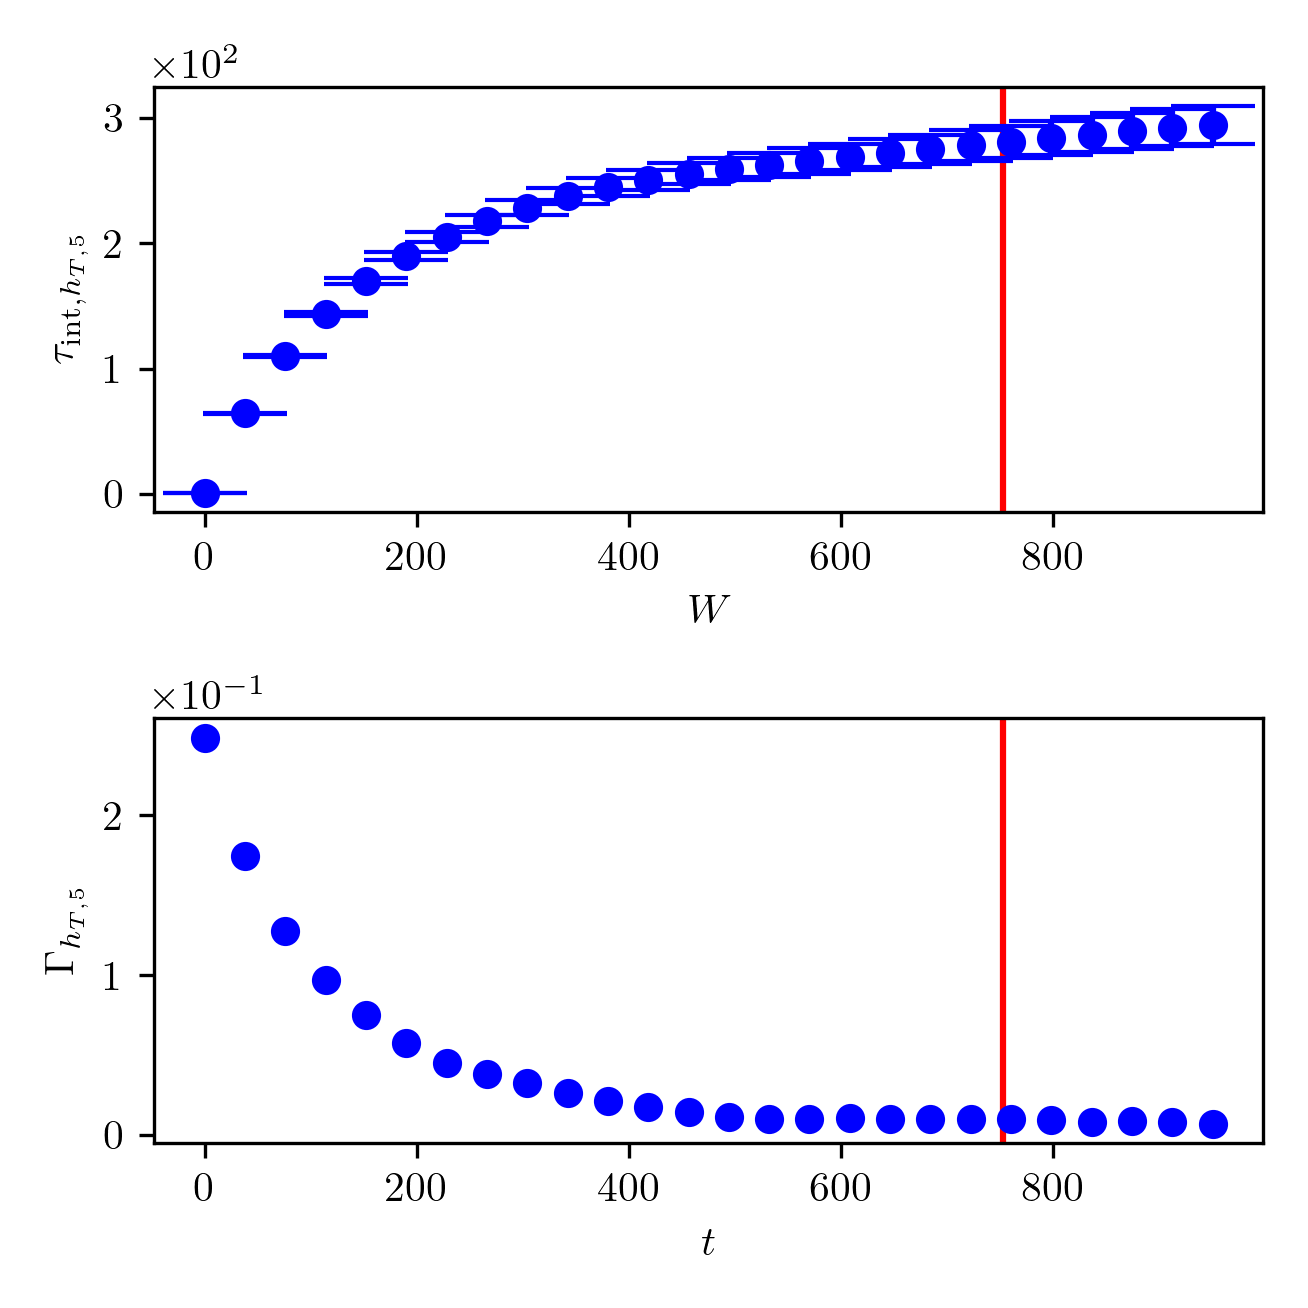
\includegraphics{UwerrTauIntTWalk14.png}
	\caption[IACT and autocorrelation function of samples $h_{T,5} \sim \pi(\cdot|\bm{y})$, for approximated model.]{Provided by \cite{drikHesse}, the IACT $\tau_{\text{int},h_{T,5}}$ at summation windows W and the estimated autocorrelation function $\Gamma_{h_{T,5}}$ at lag $t$ of samples $h_{T,5} \sim \pi( \cdot| \bm{y})$ from the t-walk for the approximated forward model.}
	\label{fig:TWalkIATC15}
\end{figure}

\begin{figure}[ht!]
	\centering
	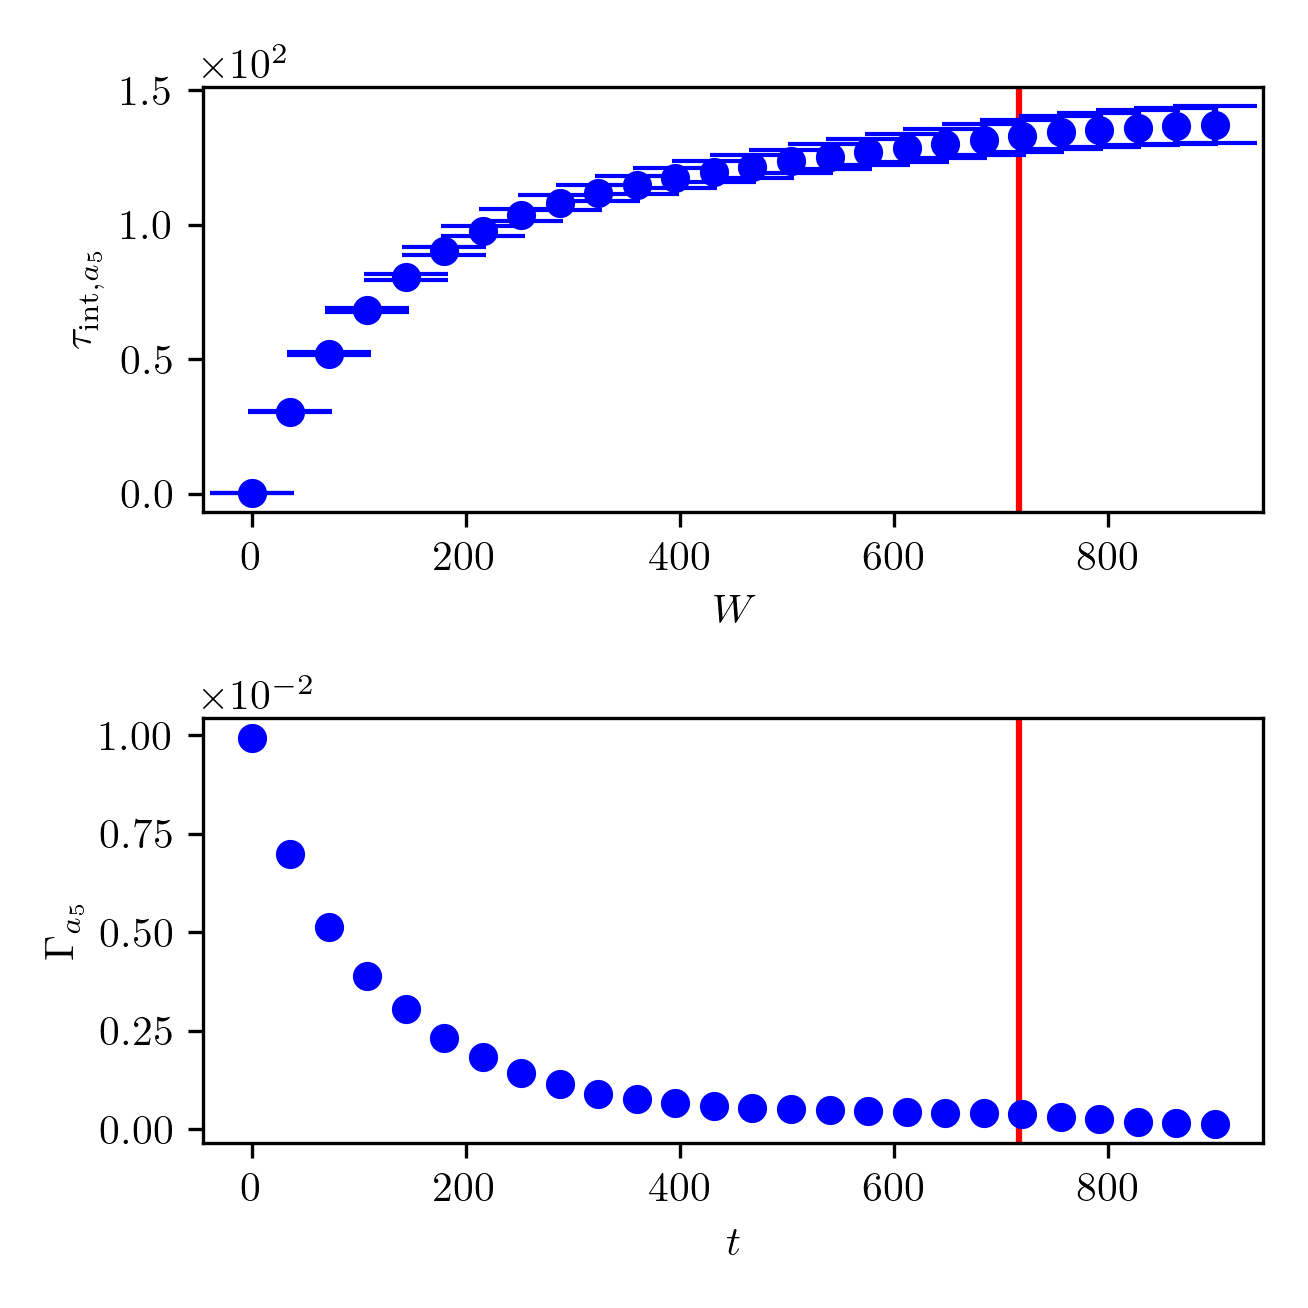
\includegraphics{UwerrTauIntTWalk15.png}
	\caption[IACT and autocorrelation function of samples $a_5 \sim \pi(\cdot|\bm{y})$, for approximated model.]{Provided by \cite{drikHesse}, the IACT $\tau_{\text{int},a_5}$ at summation windows W and the estimated autocorrelation function $\Gamma_{a_5}$ at lag $t$ of samples $a_5 \sim \pi(\cdot| \bm{y})$ from the t-walk for the approximated forward model.}
	\label{fig:TWalkIATC16}
\end{figure}
\begin{figure}[ht!]
	\centering
	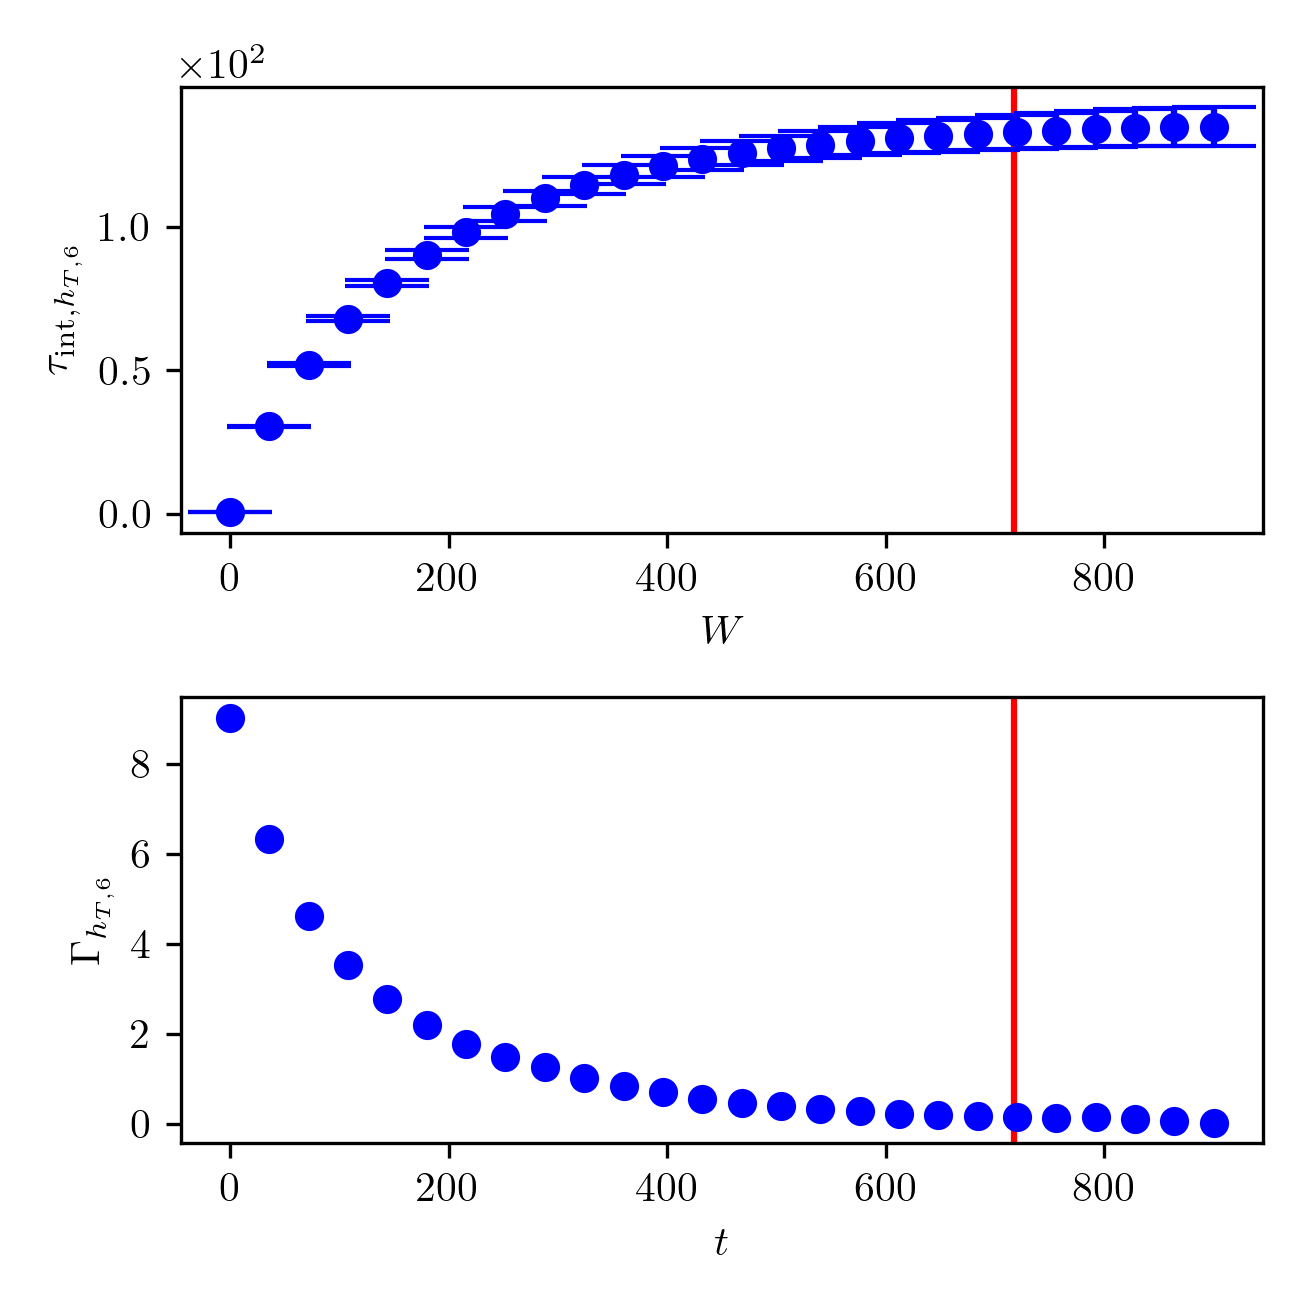
\includegraphics{UwerrTauIntTWalk16.png}
	\caption[IACT and autocorrelation function of samples $h_{T,6} \sim \pi(\cdot|\bm{y})$, for approximated model.]{Provided by \cite{drikHesse}, the IACT $\tau_{\text{int},h_{T,6}}$ at summation windows W and the estimated autocorrelation function $\Gamma_{h_{T,6}}$ at lag $t$ of samples $h_{T,6} \sim \pi( \cdot| \bm{y})$ from the t-walk for the approximated forward model.}
	\label{fig:TWalkIATC17}
\end{figure}

\begin{figure}[ht!]
	\centering
	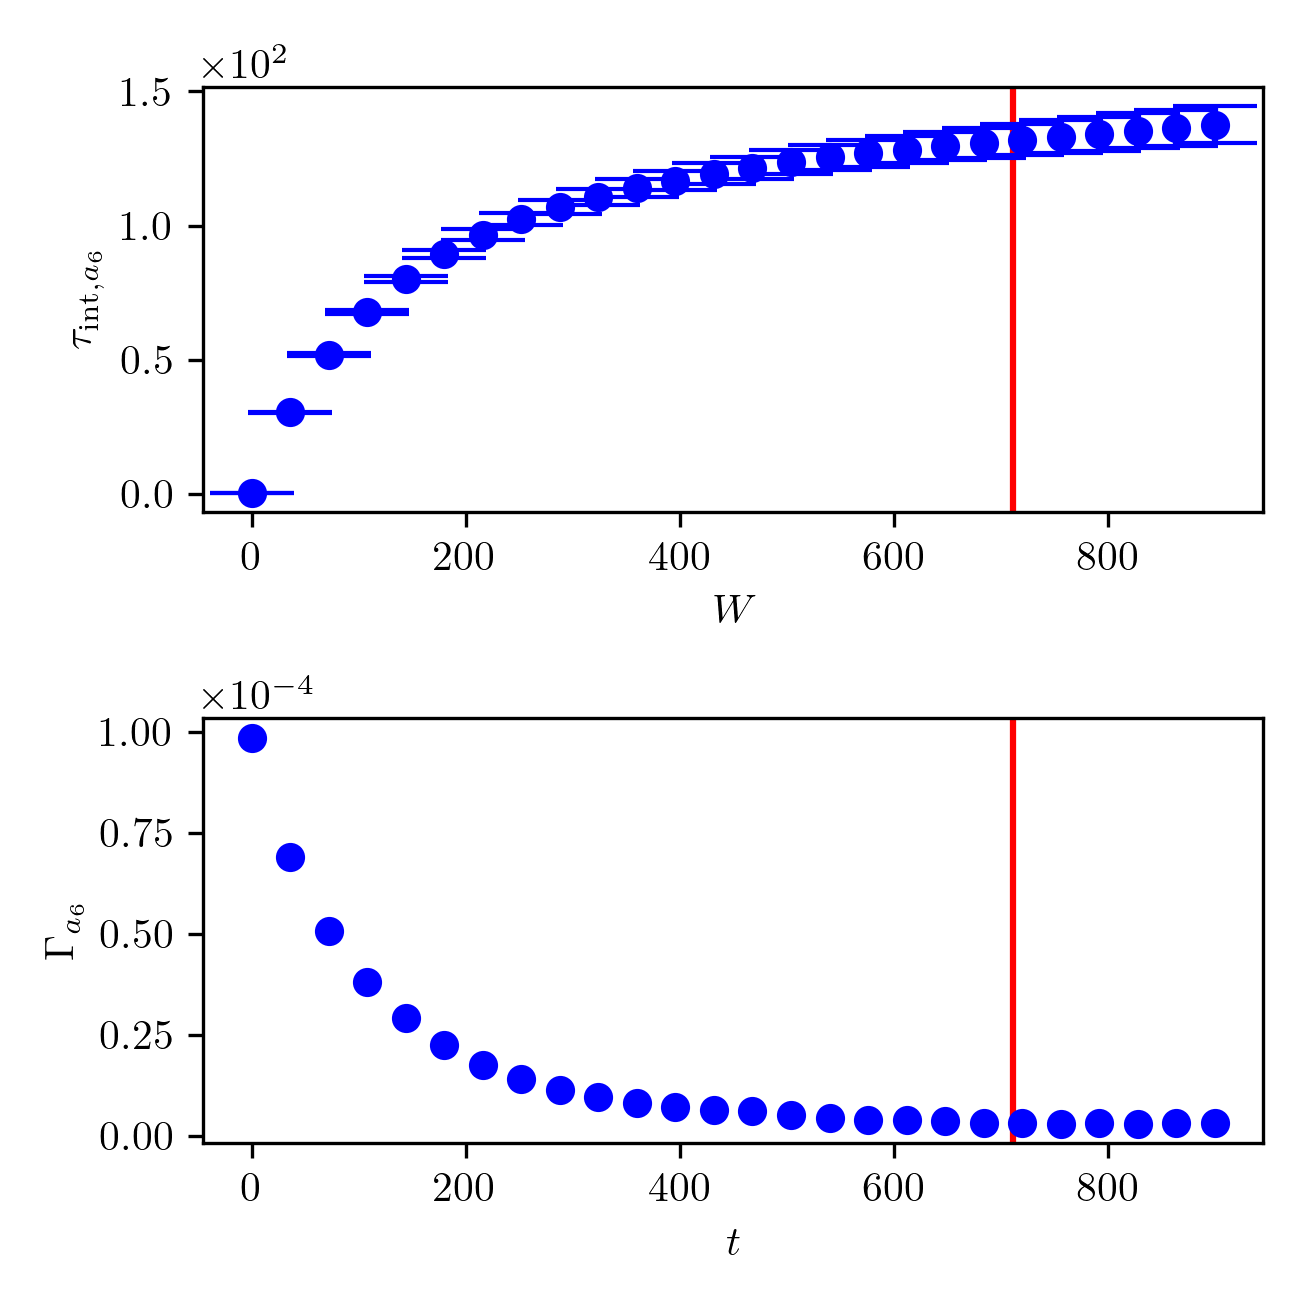
\includegraphics{UwerrTauIntTWalk17.png}
	\caption[IACT and autocorrelation function of samples $a_6 \sim \pi(\cdot|\bm{y})$, for approximated model.]{Provided by \cite{drikHesse}, the IACT $\tau_{\text{int},a_6}$ at summation windows W and the estimated autocorrelation function $\Gamma_{a_6}$ at lag $t$ of samples $a_6 \sim \pi( \cdot| \bm{y})$ from the t-walk for the approximated forward model.}
	\label{fig:TWalkIATC18}
\end{figure}





